%% Developers manual for C++ BOUT code

\documentclass[12pt]{article}
\usepackage[nofoot]{geometry}
\usepackage{graphicx}
\usepackage{fancyhdr}

\usepackage{listings}
\usepackage{color}
\usepackage{textcomp}
\definecolor{listinggray}{gray}{0.9}
\definecolor{lbcolor}{rgb}{0.95,0.95,0.95}
\lstset{
	backgroundcolor=\color{lbcolor},
        language=C++,
	keywordstyle=\bfseries\ttfamily\color[rgb]{0,0,1},
	identifierstyle=\ttfamily,
	commentstyle=\color[rgb]{0.133,0.545,0.133},
	stringstyle=\ttfamily\color[rgb]{0.627,0.126,0.941},
	showstringspaces=false,
	basicstyle=\small,
	numberstyle=\footnotesize,
	numbers=left,
	stepnumber=1,
	numbersep=10pt,
	tabsize=2,
	breaklines=true,
	prebreak = \raisebox{0ex}[0ex][0ex]{\ensuremath{\hookleftarrow}},
	breakatwhitespace=false,
	aboveskip={0.5\baselineskip},
        columns=fixed,
        upquote=true,
        extendedchars=true,
        morekeywords={Field2D,Field3D,Vector2D,Vector3D,real,FieldGroup},
}

%% Modify margins
\addtolength{\oddsidemargin}{-.25in}
\addtolength{\evensidemargin}{-.25in}
\addtolength{\textwidth}{0.5in}
\addtolength{\textheight}{0.25in}
%% SET HEADERS AND FOOTERS

\pagestyle{fancy}
\fancyfoot{}
\renewcommand{\sectionmark}[1]{         % Lower case Section marker style
  \markright{\thesection.\ #1}}
\fancyhead[LE,RO]{\bfseries\thepage}    % Page number (boldface) in left on even
                                        % pages and right on odd pages 
\renewcommand{\headrulewidth}{0.3pt}

\newcommand{\code}[1]{\texttt{#1}}
\newcommand{\file}[1]{\texttt{\bf #1}}

%% commands for boxes with important notes
\newlength{\notewidth}
\addtolength{\notewidth}{\textwidth}
\addtolength{\notewidth}{-3.\parindent}
\newcommand{\note}[1]{
\fbox{
\begin{minipage}{\notewidth}
{\bf NOTE}: #1
\end{minipage}
}}

\newcommand{\pow}{\ensuremath{\wedge} }
\newcommand{\poweq}{\ensuremath{\wedge =} }

\newcommand{\deriv}[2]{\ensuremath{\frac{\partial #1}{\partial #2}}}

\newcommand{\rbtsq}{\ensuremath{\left(RB_\theta\right)^2}}
\newcommand{\sbt}{\ensuremath{\sigma_{B\theta}}}
\newcommand{\apar}{\ensuremath{A_{||}}}
\newcommand{\Bthe}{\ensuremath{B_\theta}}
\newcommand{\Bzeta}{\ensuremath{B_\zeta}}
\newcommand{\hthe}{\ensuremath{h_\theta}}

\begin{document}

\title{BOUT++ Developers' Manual}
\author{B.Dudson, University of York}

\maketitle

\tableofcontents

\section{Introduction}

This is a manual describing the core BOUT++ code, and is intended for anyone who
wants to work on improving BOUT++. It does its best to describe
the details of how BOUT++ works, and assumes that the user is very comfortable
with C++. For a general introduction, and instructions for using BOUT++
see the users' guide. The user's guide assumes only minimal knowledge of C++,
and provides only those details needed to use BOUT++. 

Since BOUT++ is a scientific code, it is constantly changing and (hopefully)
being improved. This provides a moving target for documentation, and means
that describing all the details of how BOUT++ works in one document is probably
impossible. This is particularly true since often our first priority is to
write papers and code - not documentation - and so whatever is documented
is likely to be slightly out of date. A source of up-to-date documentation
of the BOUT++ code is the comments and Doxygen tags: running \code{doxygen}
on the source should produce a set of HTML documentation. See
\file{www.doxygen.org} for more details.

\subsection{Using the BOUT++ repository}

As of June 2009, the BOUT++ distribution is hosted on Github:

\file{http://github.com/bendudson/BOUT/}

If you're just starting with BOUT++, current developers will want to check
your changes before submitting them to the repository. In this case
you should clone (checkout) the git repository, make any changes and
then submit patches to one of the developers (e.g.
to \texttt{bd512@york.ac.uk}). Fortunately Git makes this process quite easy:
First get a copy of BOUT++
\begin{verbatim}
$ git clone git://github.com/bendudson/BOUT.git
\end{verbatim}
The BOUT++ repository will now be in a directory called ``BOUT''
(sorry - github doesn't like '+' in project names). To get the latest
changes (\code{svn update} equivalent), use
\begin{verbatim}
$ git pull
\end{verbatim}
To see the status of the repository, commits etc. use 
\begin{verbatim}
$ gitk
\end{verbatim}
This is also useful for showing what changes you've made which need to be
committed, or which haven't yet been sent to the main repository.

You can make edits as normal, and commit them using
\begin{verbatim}
$ git commit -a
\end{verbatim}
which is pretty much the equivalent of \code{svn commit} in that
it commits all changes, though importantly it doesn't send them to
a central server. To see which changes will be committed, use
\begin{verbatim}
$ git status
\end{verbatim}
To choose which files you want to commit, use 
\begin{verbatim}
$ git add file1, file2, ...
$ git commit
\end{verbatim}
(Git can actually only commit selected parts of files if you want). To 
make using Git easier, you can create a config file \file{\$HOME/.gitconfig}
containing:
\begin{lstlisting}[language=bash,numbers=none]
[user]
	name = Ben Dudson
	email = bd512@york.ac.uk

[alias]
	st = status
	ci = commit
	br = branch
	co = checkout
	df = diff
	lg = log -p
	who = shortlog -s --
\end{lstlisting}
(though obviously you should change the name and email).

Once you're done making changes, you should first pull the latest changes
from the server:
\begin{verbatim}
$ git pull
\end{verbatim}
{\bf Read carefully} what git prints out. If there are conflicts
then git will try to resolve them, but in some cases you will have 
to resolve them yourself. To see a list of conflicting changes
run \code{git status} (or \code{git st} if you're using the above
\file{.gitconfig} file). Once you've finished resolving conflicts,
run \code{git commit -a} to commit the merge.

After you've got the latest changes, and resolved conflicts, create
a patch:
\begin{verbatim}
$ git format-patch origin/master --stdout > your-patch-file.diff
\end{verbatim}
Now you can email this patch to someone who can commit to the Git archive
(e.g. Ben Dudson, bd512@york.ac.uk).

If you are doing a lot of development of BOUT++, it will probably make sense
for you to push changes directly to the online repository. 
In this case you'll need to sign up for an account on \file{github.com},
then upload an ssh key and ask to be added. The process is
then almost identical except that you clone using SSH:
\begin{verbatim}
$ git clone git@github.com:bendudson/BOUT.git
\end{verbatim}
and rather than creating a patch, you push changes to the repository:
\begin{verbatim}
$ git push
\end{verbatim}

\subsection{House rules}

BOUT++ consists of about 31,800 lines of C/C++\footnote{generated using
David A. Wheeler's 'SLOCCount'},
along with 11,600 lines of IDL. Of this, about 21,100 lines is the core
BOUT++ code, and the remainder
a mix of pre- and post-processors, and physics modules. As production codes
go, this is not particularly huge, but it is definitely large enough that
keeping the code `clean' and understandable is necessary. This is vital
if many people are going to work on the code, and also greatly helps code
debugging and verification. There are therefore a few house rules to keep
in mind when modifying the BOUT++ code.

When modifying the core BOUT++ code, please keep in mind that this portion of the code
is intended to be general (i.e. independent of any particular physical system of equations),
and to be used by a wide range of users. Making code clear is also more important
in this section than the physics model since the number of developers is potentially
much greater. 

Here are some rules for editing the core BOUT++ code:
\begin{itemize}
\item {\bf NO FORTRAN}. EVER. Though it may be tempting for scientific programmers to use
a little FORTRAN now and then, please please don't put any into BOUT++. 
Use of FORTRAN, particularly when mixed with C/C++, is the cause of many problems in
porting and modifying codes. 
\item If a feature is needed to study a particular system, only include it in the
core code if it is more generally applicable, or cannot be put into the physics module.
\end{itemize}

\subsection{Naming conventions}

The naming of BOUT++ classes, functions etc. has not been very consistent
historically, but please try to follow the following rules:
\begin{itemize}
\item Directories and files are all lower case (with underscores)
\item Class names start with a capital letter, and each word is capitalised e.g. \code{BoutMesh}. No underscores.
\item Class member functions start with a lower case letter with each subsequent word capitalised (e.g. \code{write()}, \code{setSection()}), also without underscores.
\item Variable names are all lower case, with underscores if you want.
\end{itemize}

\section{Code layout}

BOUT++ is organised into classes and groups of functions which operate on them: 
It's not purely object-oriented, but takes advantage of many of C++'s object-oriented features. 

Figure~\ref{fig:layout1} shows the most important parts of BOUT++ and how they fit together.
\begin{figure}[htbp!]
\centering
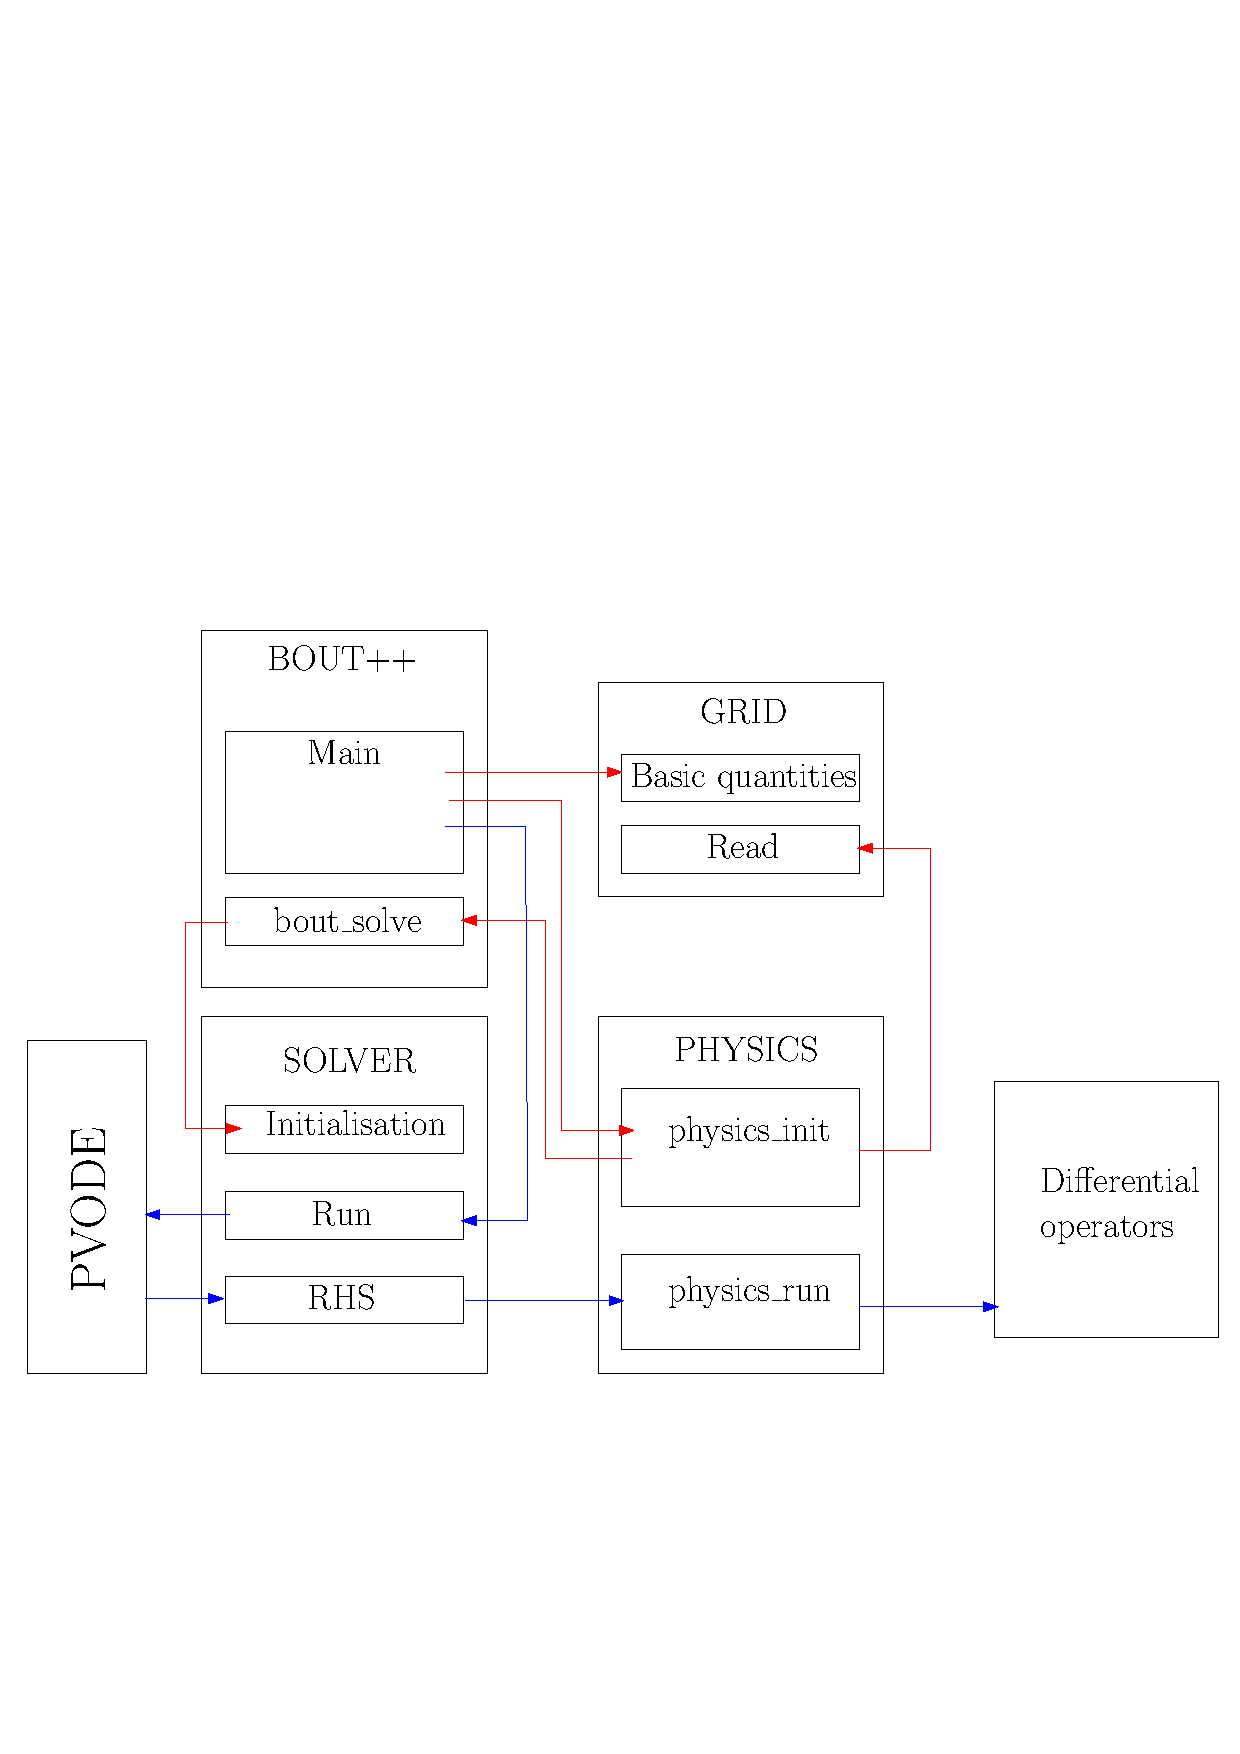
\includegraphics[width=0.7\paperwidth, keepaspectratio]{figs/layout1.pdf}
\caption{Overview of BOUT++ control flow during initialisation (red), and running (blue)}
\label{fig:layout1}
\end{figure}
The initialisation process is shown in red: basic information is first read from the grid
file (e.g. size of the grid, topology etc.), then the user-supplied initialisation
code is called. This code can read other variables from the grid, and makes at least
one call
to \code{bout\_solve} to specify a variable to be evolved. The main thing \code{bout\_solve}
does is to add these variables to the solver. 

The process of running a timestep is shown in blue in figure~\ref{fig:layout1}:
The main loop calls the solver, which in turn calls PVODE. To evolve the system
PVODE makes calls to the RHS function inside solver. This moves data between PVODE
and BOUT++, and calls the user-supplied \code{physics\_run} code to calculate
time-derivatives. Much of the work calculating time-derivatives involves differential
operators.

Calculation of the RHS function \code{physics\_run}, and handling of data
in BOUT++ involves many different components. Figure~\ref{fig:layout2}
shows (most) of the classes and functions involved, and the relationships
between them. Some thought was put into how this should be organised, but
it has also changed over time, so some parts could be cleaner.
\begin{figure}[htbp!]
\centering
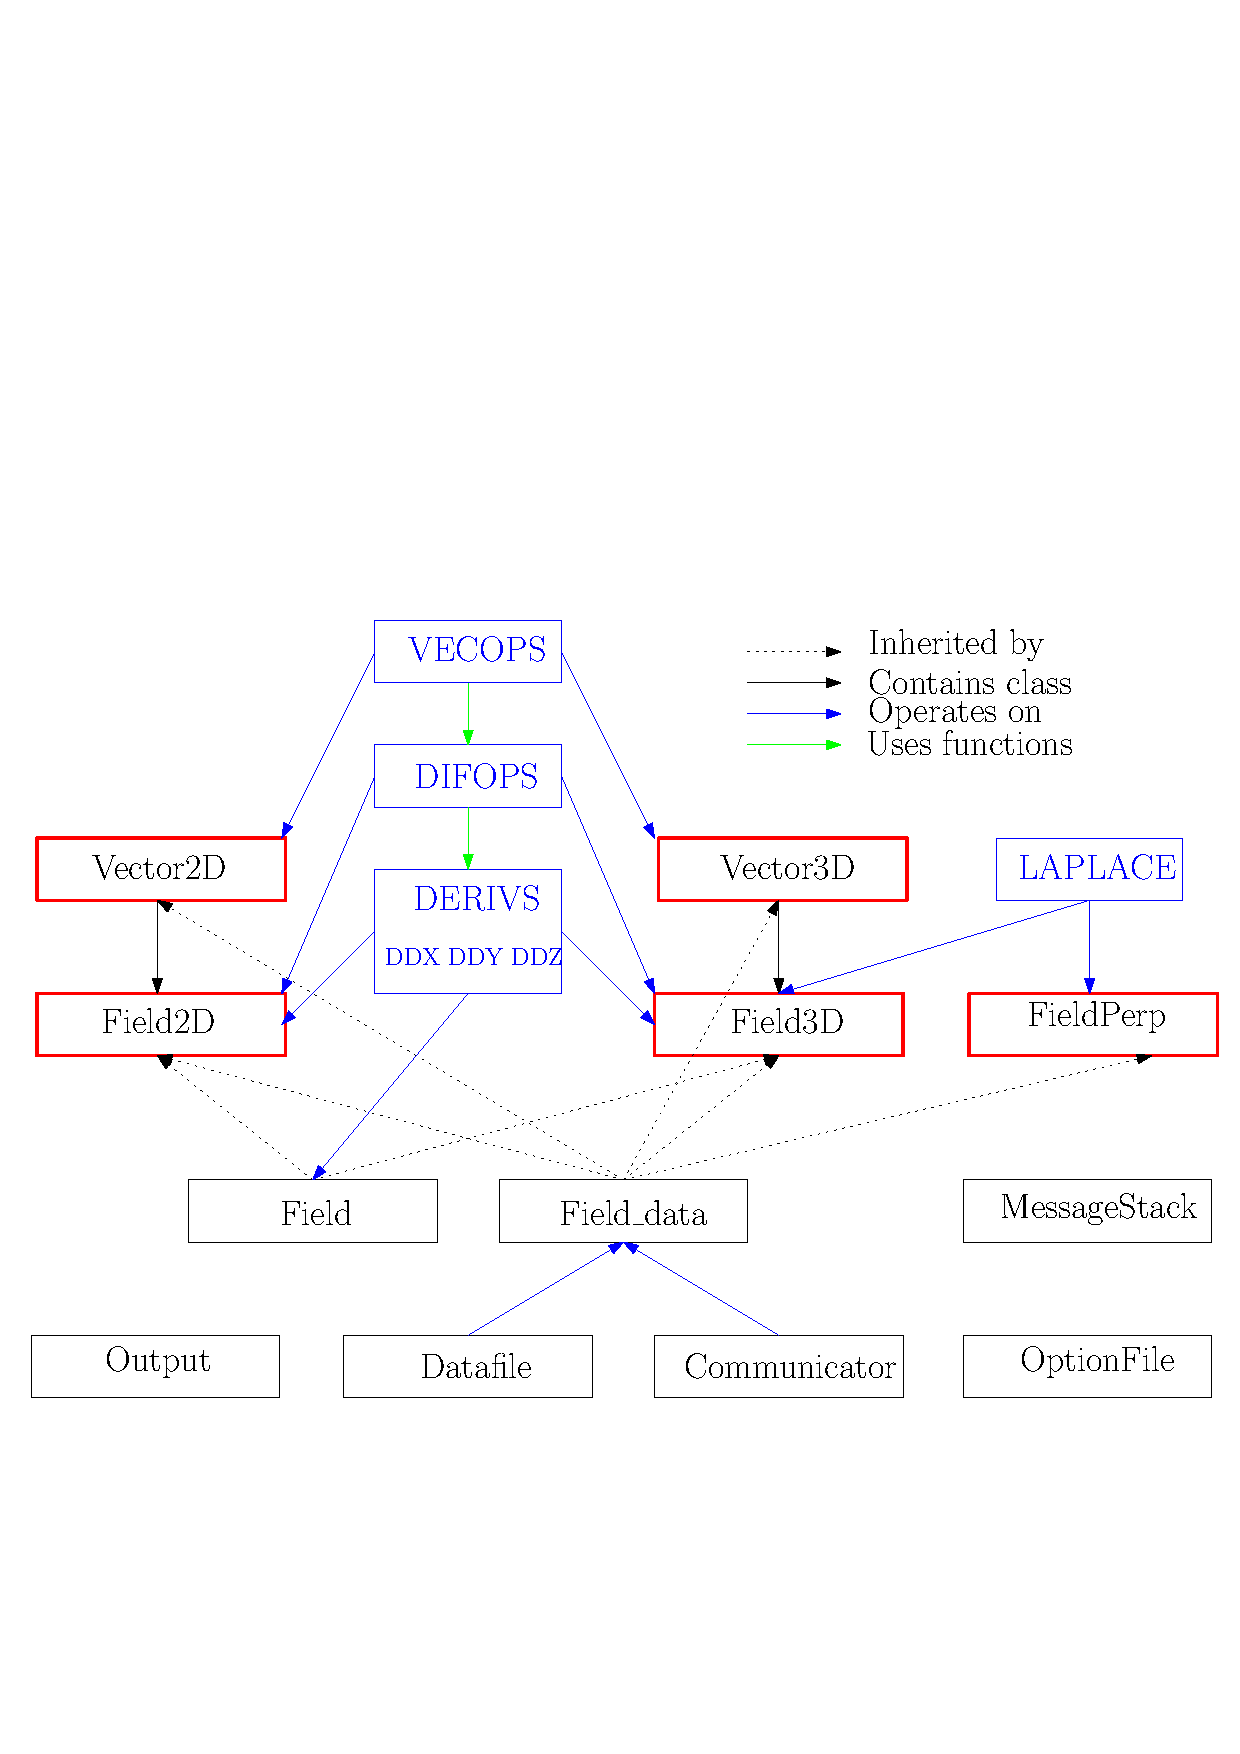
\includegraphics[width=0.6\paperwidth, keepaspectratio]{figs/layout2.pdf}
\caption{Relationship between important classes and functions used in calculating the RHS function}
\label{fig:layout2}
\end{figure}

\subsection{Directories}

The source code for the core of BOUT++ is divided into
include files (which can be used in physics models) in 
\file{bout++/include}, and source code and low-level includes
in \file{bout++/src}. Inside \file{bout++/src}, the current source code
files are:
\begin{itemize}
\item \file{bout++.cpp} : Main file which initialises, runs and finalises
  BOUT++. Currently contains a \code{main()} function, though this is
  being removed shortly.
\item field
  \begin{itemize}
  \item \file{field2d.cpp} implements the \code{Field2D} class. This is a
    scalar field which varies only in $x$ and $y$ and is used for things
    like metric tensor components and initial profiles. It supplies lots
    of overloaded operators and functions on these objects.
  \item \file{field3d.cpp} implements the \code{Field3D} class, which varies 
    in $x$, $y$ and $z$. Since these handle a lot more memory than Field2D
    objects, the memory management is more complicated and includes reference
    counting. See section~\ref{sec:memorymanage} for more details.
  \item \file{field\_data.cpp} Implements some functions in the \code{FieldData} class. This is a mainly pure virtual interface class which is inherited by \code{Field2D} and \code{Field3D}.
  \item \file{fieldperp.cpp} implements a \code{FieldPerp} class to store
    slices perpendicular to the magnetic field i.e. they are a function of
    $x$ and $z$ only. This is mainly used for Laplacian inversion routines,
    and needs to be integrated with the other fields better.
  \item \file{initialprofiles.cpp} routines to set the initial values of
    fields when a simulation first starts. Reads settings from the option
    file based on the name of the variable.
  \item \file{vecops.cpp} a collection of function to operate on vectors. 
    Contains things like \code{Grad}, \code{Div} and \code{Curl}, and uses
    a combination of field differential operators (in \file{difops.cpp}) and
    metric tensor components (in \code{Mesh}).
  \item \file{vector2d.cpp} implements the \code{Vector2D} class, which uses
    a \code{Field2D} object for each of its 3 components. Overloads operators 
    to supply things like dot and cross products.
  \item \file{vector3d.cpp} implements \code{Vector3D} by using a
    \code{Field3D} object for each component.
  \item \file{where.cpp} supplies functions for choosing between values
    based on selection criteria.
  \end{itemize}
\item fileio
  \begin{itemize}
  \item \file{datafile.cpp} supplies an abstract \code{DataFile} interface
    for data input and output. Handles the conversion of data in fields
    and vectors into blocks of data which are then sent to a specific file
    format.
  \item \file{nc\_format.cpp} implements an interface to the NetCDF-4 library
  \item \file{nc\_format.h} is the header file. This is not in the
    \file{include/} directory because it should only be used by \code{DataFile}.
  \item \file{pdb\_format.cpp} implements an interace to Portable Data
    Binary (PDB) formatted files.
  \item \file{pdb\_format.h}
  \end{itemize}
\item invert
  \begin{itemize}
  \item \file{fft\_fftw.cpp} implements the \code{fft.h} interface by calling
    the Fastest Fourier Transform in the West (FFTW) library.
  \item \file{full\_gmres.cpp}
  \item \file{inverter.cpp} is a \code{FieldPerp} inversion class currently
    under development. It is intended to provide a way to solve nonlinear
    problems using a GMRES iterative method.
  \item \file{invert\_gmres.cpp}
  \item \file{invert\_laplace.cpp} uses Fourier decomposition in $z$ combined
    with tri- and band-diagonal solvers in $x$ to solve Laplacian problems.
  \item \file{invert\_laplace\_gmres.cpp} inherits the \code{Inverter} class
    and will solve more general Laplacian problems, using the
    \code{invert\_laplace} routines as preconditioners.
  \item \file{invert\_parderiv.cpp} inverts a problem involving only parallel
    $y$ derivatives. Intended for use in some preconditioners.
  \item \file{lapack\_routines.cpp} supplies an interface to the LAPACK linear
    solvers, which are used by the \code{invert\_laplace} routines.
  \end{itemize}
\item mesh
  \begin{itemize}
  \item \file{boundary\_factory.cpp} creates boundary condition operators
    which can then be applied to fields. Described in
    section~\ref{sec:BoundaryFactory}.
  \item \file{boundary\_region.cpp} implements a way to describe and iterate
    over boundary regions. Created by the mesh, and then used by boundary
    conditions. See section~\ref{sec:BoundaryRegion} for more details.
  \item \file{boundary\_standard.cpp} implements some standard boundary
    operations and modifiers such as \code{Neumann} and \code{Dirichlet}.
  \item \file{boutmesh.cpp} implements a mesh interface which is compatible
    with BOUT grid files.
  \item \file{difops.cpp} is a collection of differential operators on scalar
    fields. It uses the differential methods in \file{derivs.cpp} and the
    metric tensor components in \code{Mesh} to compute operators.
  \item \file{grid.cpp} contains some routines which are used by the \code{Mesh}
    to read data. 
  \item \file{interpolation.cpp} contains functions for interpolating fields
  \item \file{mesh.cpp} is the base class for the \code{Mesh} object. Contains
    routines useful for all \code{Mesh} implementations.
  \item \file{quiltmesh.cpp} is an implementation of \code{Mesh} which is
    currently under development. It is intended to handle more general mesh
    shapes and topology than the currently used \code{BoutMesh} can handle.
  \end{itemize}
\item physics
  \begin{itemize}
  \item \file{smoothing.cpp} provides smoothing routines on scalar fields
  \item \file{sourcex.cpp} contains some useful routines for creating
    sources and sinks in physics equations.
  \end{itemize}
\item precon
  \begin{itemize}
  \item \file{jstruc.cpp} is an experimental code for preconditioning using
    PETSc
  \end{itemize}
\item solver
  \begin{itemize}
  \item \file{solver.cpp} is the interface for all solvers 
  \item \file{solverfactory.cpp} creates solver objects
  \item \file{solverfactory.h}
  \item impls
    \begin{itemize}
    \item cvode
      \begin{itemize}
      \item \file{cvode.cpp} is the implementation of \code{Solver} which
        interfaces with the SUNDIALS CVODE library.
      \item \file{cvode.h}
      \end{itemize}
    \item ida
      \begin{itemize}
      \item \file{ida.cpp} is the implementation which interfaces with the
        SUNDIALS IDA library
      \item \file{ida.h}
      \end{itemize}
    \item petsc
      \begin{itemize}
      \item \file{petsc.cpp} is the interface to the PETSc time integration
        routines
      \item \file{petsc.h}
      \end{itemize}
    \item pvode
      \begin{itemize}
      \item \file{pvode.cpp} interfaces with the 1998 (pre-SUNDIALS) version
        of PVODE (which became CVODE).
      \item \file{pvode.h}
      \end{itemize}
    \end{itemize}
  \end{itemize}
\item sys
  \begin{itemize}
  \item \file{boutexception.cpp} is an exception class which are used
    for error handling
  \item \file{comm\_group.cpp} provides routines for non-blocking collective 
    MPI operations. These are not available in MPI-2, though are planned for
    MPI-3.
  \item \file{dcomplex.cpp} provides a \code{dcomplex} complex type. It is here
    because the original type \code{real} conflicted with the STL definition.
    This could probably be replaced with the STL implementation now.
  \item \file{derivs.cpp} contains basic derivative methods such as
    upwinding, central difference and WENO methods. These are then
    used by \file{difops.cpp}. Details are given in
    section~\ref{sec:derivatives}.
  \item \file{diagnos.cpp} is the start of a diagnostics code which will extract
    values from fields each timestep and print to the output log file. Not
    yet finished.
  \item \file{msg\_stack.cpp} is part of the error handling system. It maintains
    a stack of messages which can be pushed onto the stack at the start of 
    a function, then removed (popped) at the end. If an error occurs or 
    a segmentation fault is caught then this stack is printed out and can
    help to find errors.
  \item \file{options.cpp} provides an interface to the BOUT.inp option file
    and the command-line options. 
  \item \file{stencils.cpp} contains methods to operate on stencils which are
    used by differential methods. 
  \item \file{utils.cpp} contains miscellaneous small useful routines
    such as allocating and freeing arrays.
  \end{itemize}
\end{itemize}



\section{Data types}

The classes outlines in red in figure~\ref{fig:layout2} are data types 
currently implemented in BOUT++. 

\subsection{\code{FieldData}}

All BOUT++ data types implement a standard interface for accessing their
data, which is then used in communication and file I/O code. This interface
is in \file{src/field/field\_data.h}. The mandatory (pure virtual) functions are:
\begin{lstlisting}
bool isReal(); // Returns true if field consists of real values
bool is3D() const;   // True if variable is 3D
  
int byteSize() const; // Number of bytes for a single point
int realSize() const; // Number of reals (not implemented if not real)
  
int getData(int x, int y, int z, void *vptr) const; // Return number of bytes
int getData(int x, int y, int z, real *rptr) const; // Return number of reals
  
int setData(int x, int y, int z, void *vptr);
int setData(int x, int y, int z, real *rptr);
\end{lstlisting}

To support file I/O there are also some additional functions which may be implemented.
A code can check if they are implemented by calling \code{ioSupport}. If one of them
is implemented then they all should be.
\begin{lstlisting}
bool  ioSupport();  // Return true if these functions are implemented
const string getSuffix(int component) const; // For vectors e.g. "_x"
void* getMark() const; // Store current settings (e.g. co/contra-variant)
void  setMark(void *setting); // Return to the stored settings
real* getData(int component); 
void  zeroComponent(int component); // Set a component to zero
\end{lstlisting}  

For twist-shift conditions, the optional function \code{shiftZ} is called in the communication
routines.
\begin{lstlisting}
void shiftZ(int jx, int jy, double zangle);
\end{lstlisting}

\subsection{\code{Field}}

The two main types are \code{Field2D}, and \code{Field3D}. Their main functions
are to provide an easy way to manipulate data; they take care of all memory management,
and most looping over grid-points in algebraic expressions. The 2D field implementation
is relatively simple, but more optimisations are used in the 3D field implementation
because they are much larger (factor of $\sim 100$).

To handle time-derivatives, and enable expressions to be written in the
following form:
\begin{lstlisting}
ddt(Ni) = -b0xGrad_dot_Grad(phi, Ni);
\end{lstlisting}
fields (and vectors, see below) have a function:
\begin{lstlisting}
Field3D* timeDeriv();
\end{lstlisting}
which returns a pointer to the field holding the time-derivative
of this variable. This function ensures that this field is unique
using a singleton pattern.

\subsection{\code{Vector}}

Vector classes build on the field classes, just using a field to represent
each component. 

\subsection{\code{dcomplex}}

Several parts of the BOUT++ code involve FFTs and are therefore much easier to
write using complex numbers. Unfortunately, the C++ complex library also tries
to define a \code{real} type, which is already defined by PVODE. Several
work-arounds were tried, some of which worked on some systems, but
it was easier in the end to just implement a new class \code{dcomplex} to
handle complex numbers.

\subsection{Memory management}
\label{sec:memorymanage}

This code has been thoroughly tested/debugged, and should only be altered
with great care, since just about every other part of BOUT++ depends on this code
working correctly. Two optimisations used in the data objects to speed up code execution
are memory recycling, which eliminates allocation and freeing of memory; and copy-on-change,
which minimises unnecessary copying of data.

Both of these optimisations are done ``behind the scenes'', hidden from the remainder
of the code, and are illustrated in figure~\ref{fig:memory}:
\begin{figure}[htb!]
\centering
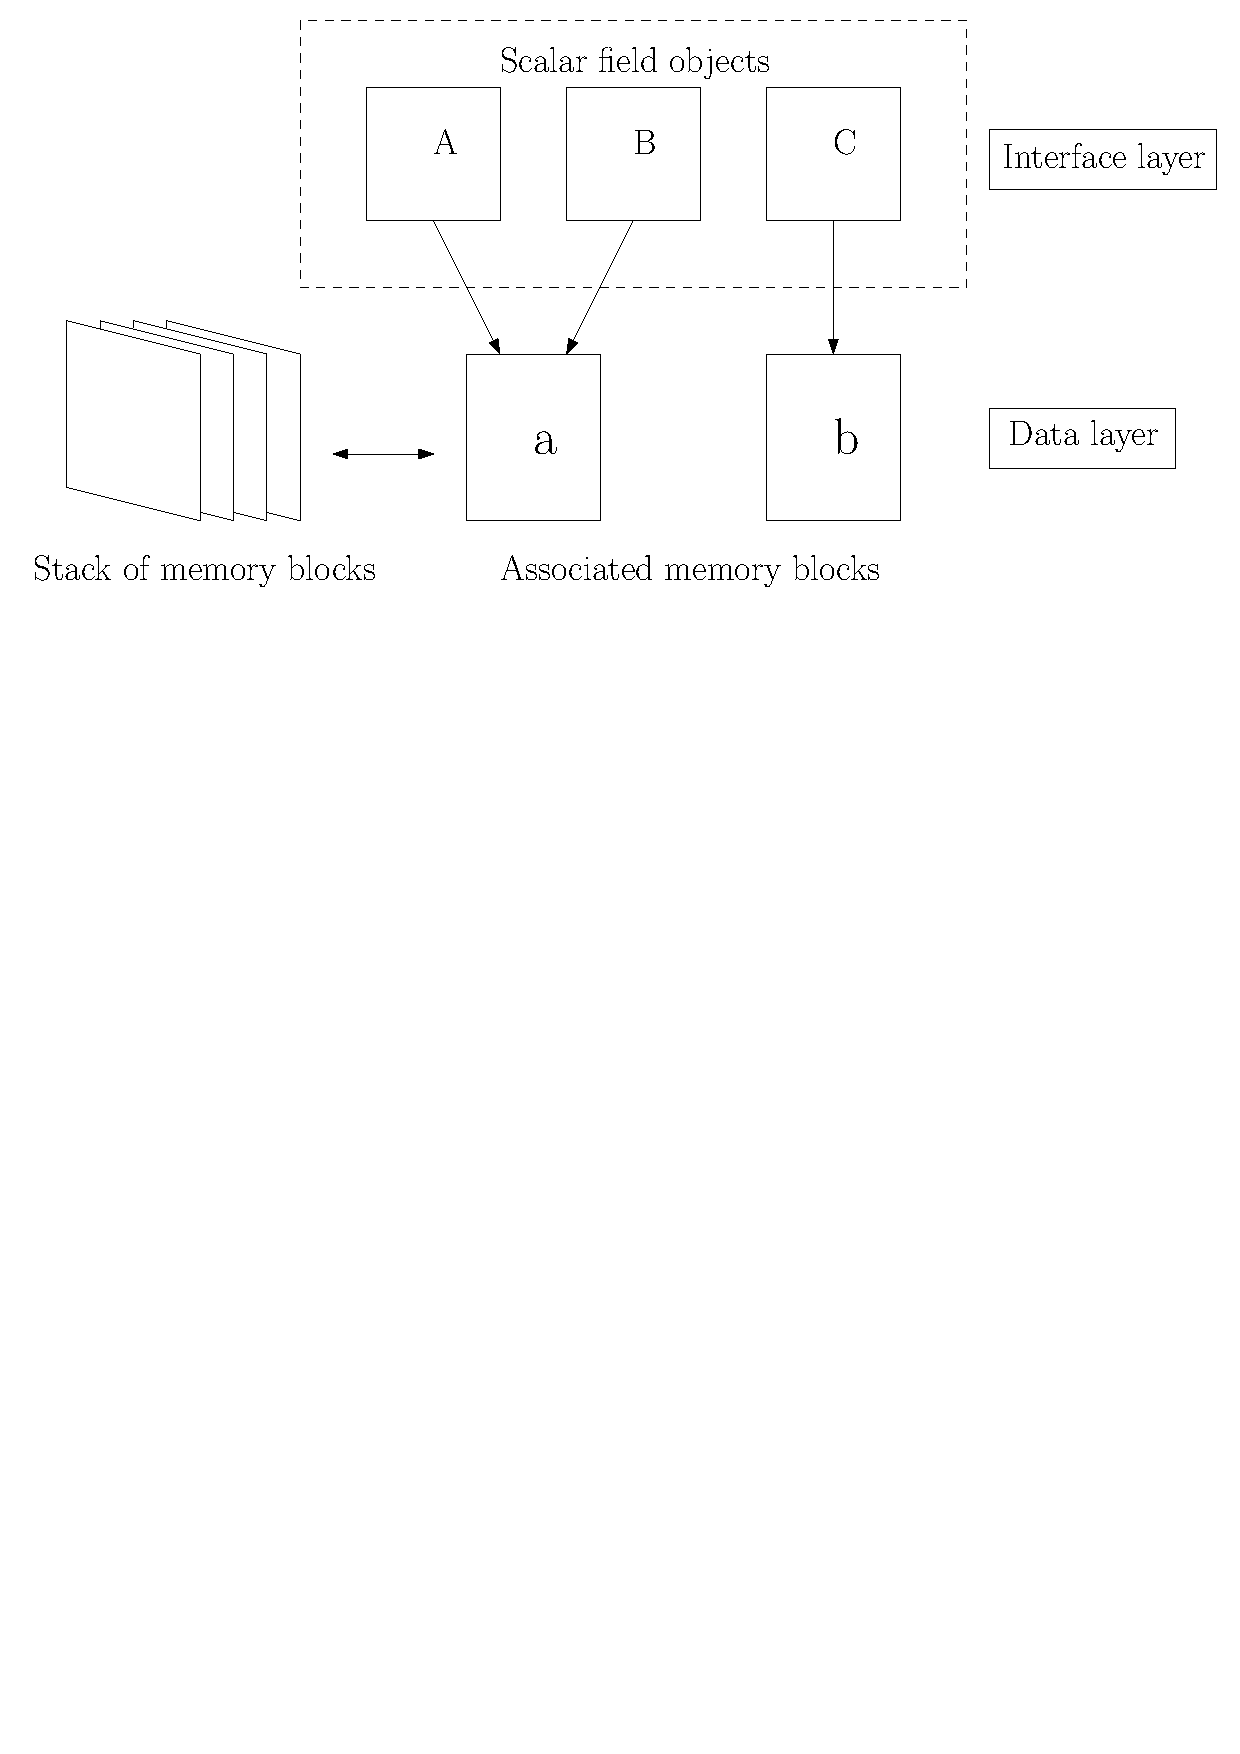
\includegraphics[scale=0.75]{figs/memory.pdf}
\caption{Memory handling in BOUT++. Memory allocation and freeing is eliminated by recycling memory blocks, and assignments without changes (\code{A = B}) do not result in copying data, only pointers to the data. Both these optimisations are handled internally, and are invisible to the programmer.}
\label{fig:memory}
\end{figure}
The objects (A,B,C) accessed by the user in operations
discussed in the previous section act as an interface to underlying data (a,b). 
Memory recycling can be used because all the scalar fields are the same size (and vector fields are
implemented as a set of 3 scalar fields). Each class implements a global stack of available
memory blocks. When an object is assigned a value, it attempts to grab one of these memory blocks,
and if none are available then a new block is allocated. 
When an object is destroyed, its memory block is not freed, but is put onto the
stack. Since the evaluation of the time-derivatives involves the same set of operations each time, this system
means that memory is only allocated the first time the time-derivatives are calculated, after which the same 
memory blocks are re-used. This eliminates the often slow system calls needed to allocate and free memory,
replacing them with fast pointer manipulation. 

Copy-on-change (reference counting) further reduces memory useage and unnecessary copying of data. 
When one field is set equal to another (e.g. \code{Field3D A = B} in figure~\ref{fig:memory}), no 
data is copied, only the reference to the underlying data (in this case both A and B point to data block a). 
Only when one of these objects is modified is a second memory block used to store the different value. 
This is particularly useful when returning objects from a routine. Usually this would
involve copying data from one object to another, and then destroying the original copy. Using
reference counting this copying is eliminated.

\note{For debugging and Valgrind output, it can be useful to disable
this memory block handling. To do this, add \code{-DDISABLE\_FREELIST} to the
compile flags}

\section{Derivatives}
\label{sec:derivatives}

This is probably the part of the code most people will want to alter. The main
task of this module is to map functions on fields like \code{DDX} to direction-independent
differential methods on stencils such as $4^{th}$-order central differencing. This mapping depends on global settings in \file{BOUT.inp}
and is illustrated in figure~\ref{fig:diffOverview}.
\begin{figure}[htb!]
\centering
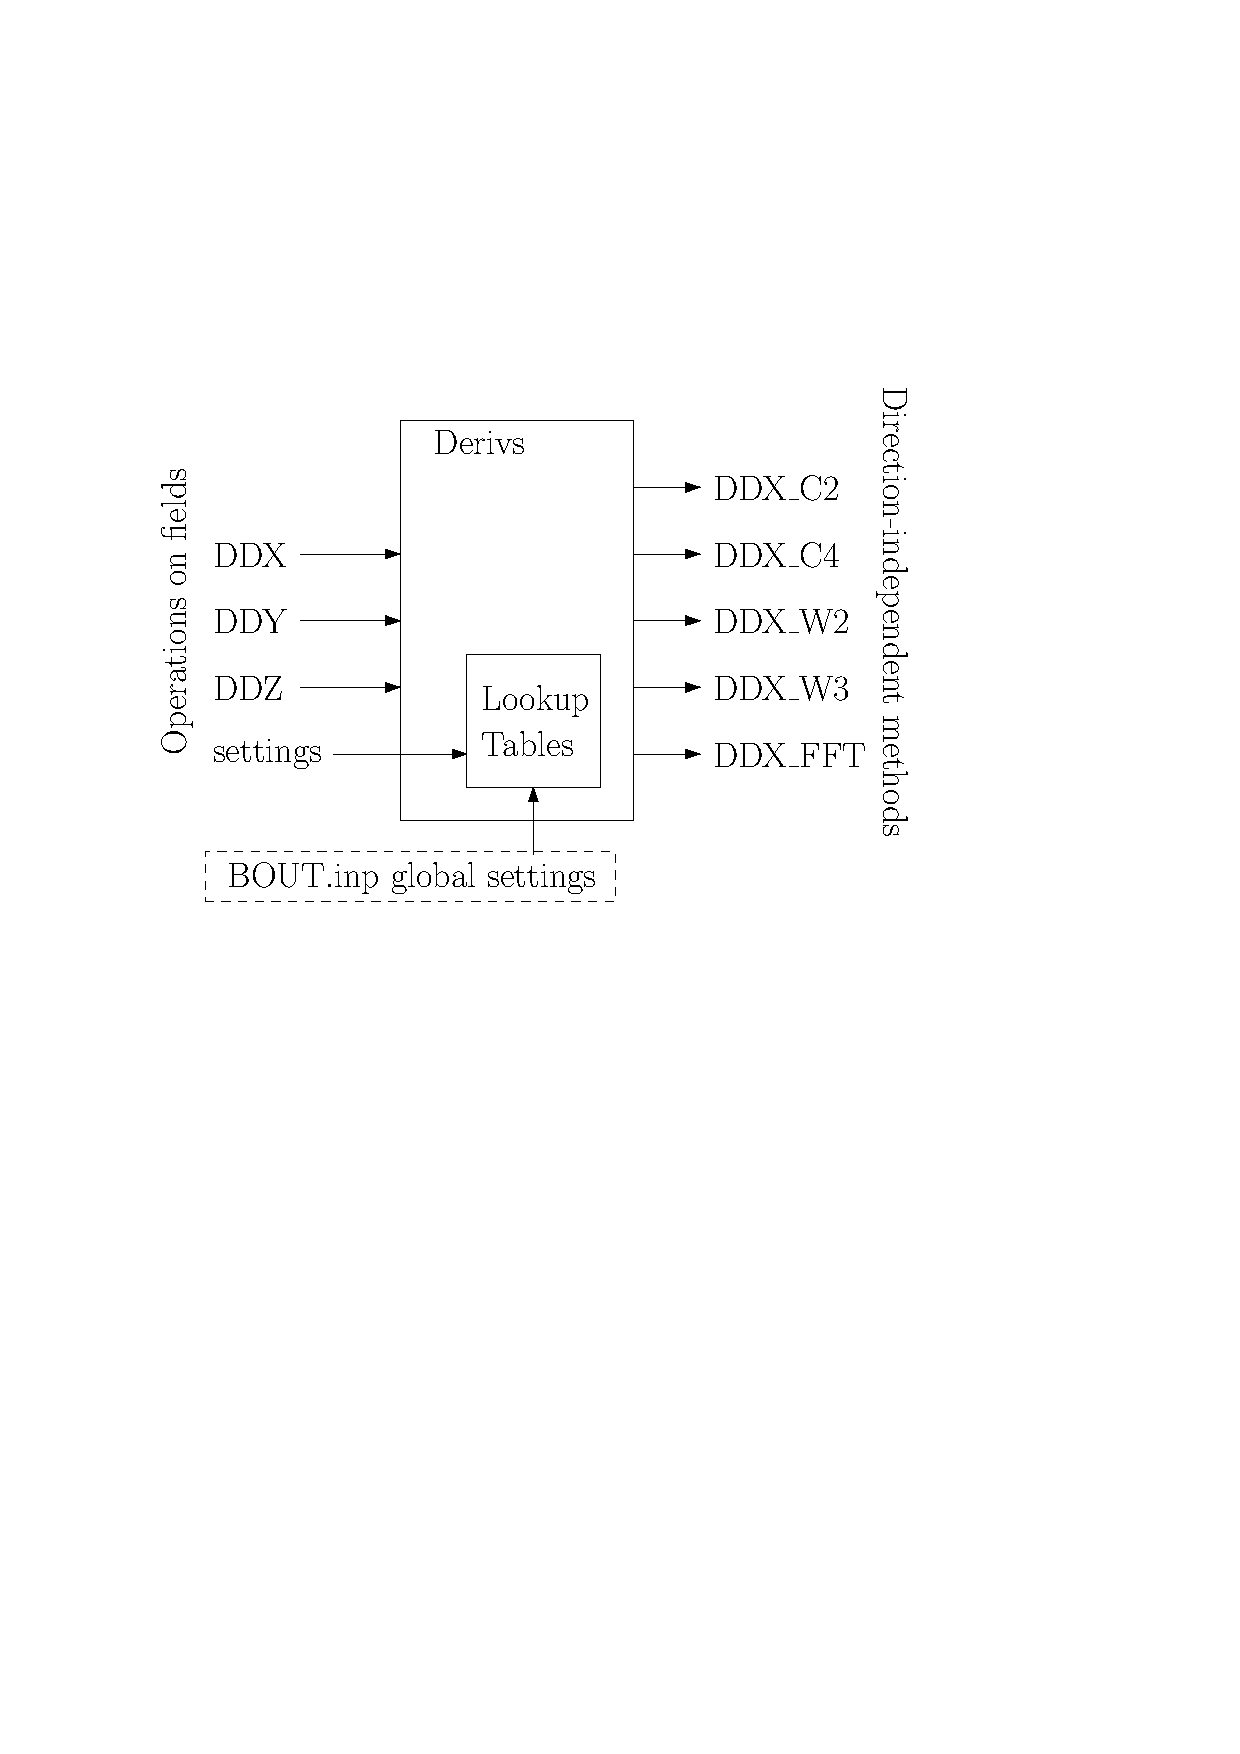
\includegraphics[scale=0.75]{figs/diffOverview.pdf}
\caption{Overview of \code{derivs} module, mapping derivative functions on fields to direction-independent differential methods}
\label{fig:diffOverview}
\end{figure}

The differencing methods themselves are independent on direction, and operate on \code{stencil}
objects. This class is in \file{stencils.h}
\begin{lstlisting}
class stencil {
  public:
    int jx, jy, jz;  // Central location
    real c, p, m, pp, mm; // stencil 2 each side of the centre
    Overloaded operators
      =,+,-,*,/
    Functions
      min, max, abs
};
\end{lstlisting}
The main purpose of this class is to store a 5-element stencil. To simplify some code
this class also has a bunch of overloaded operators on reals and other stencil objects. 
There are also some functions to calculate things like absolute, minimum, and maximum
values.

\subsection{Lookup tables}

Originally, BOUT++ used a load of \code{case} statements to determine
which differencing method to use. 

\begin{figure}[htb!]
\centering
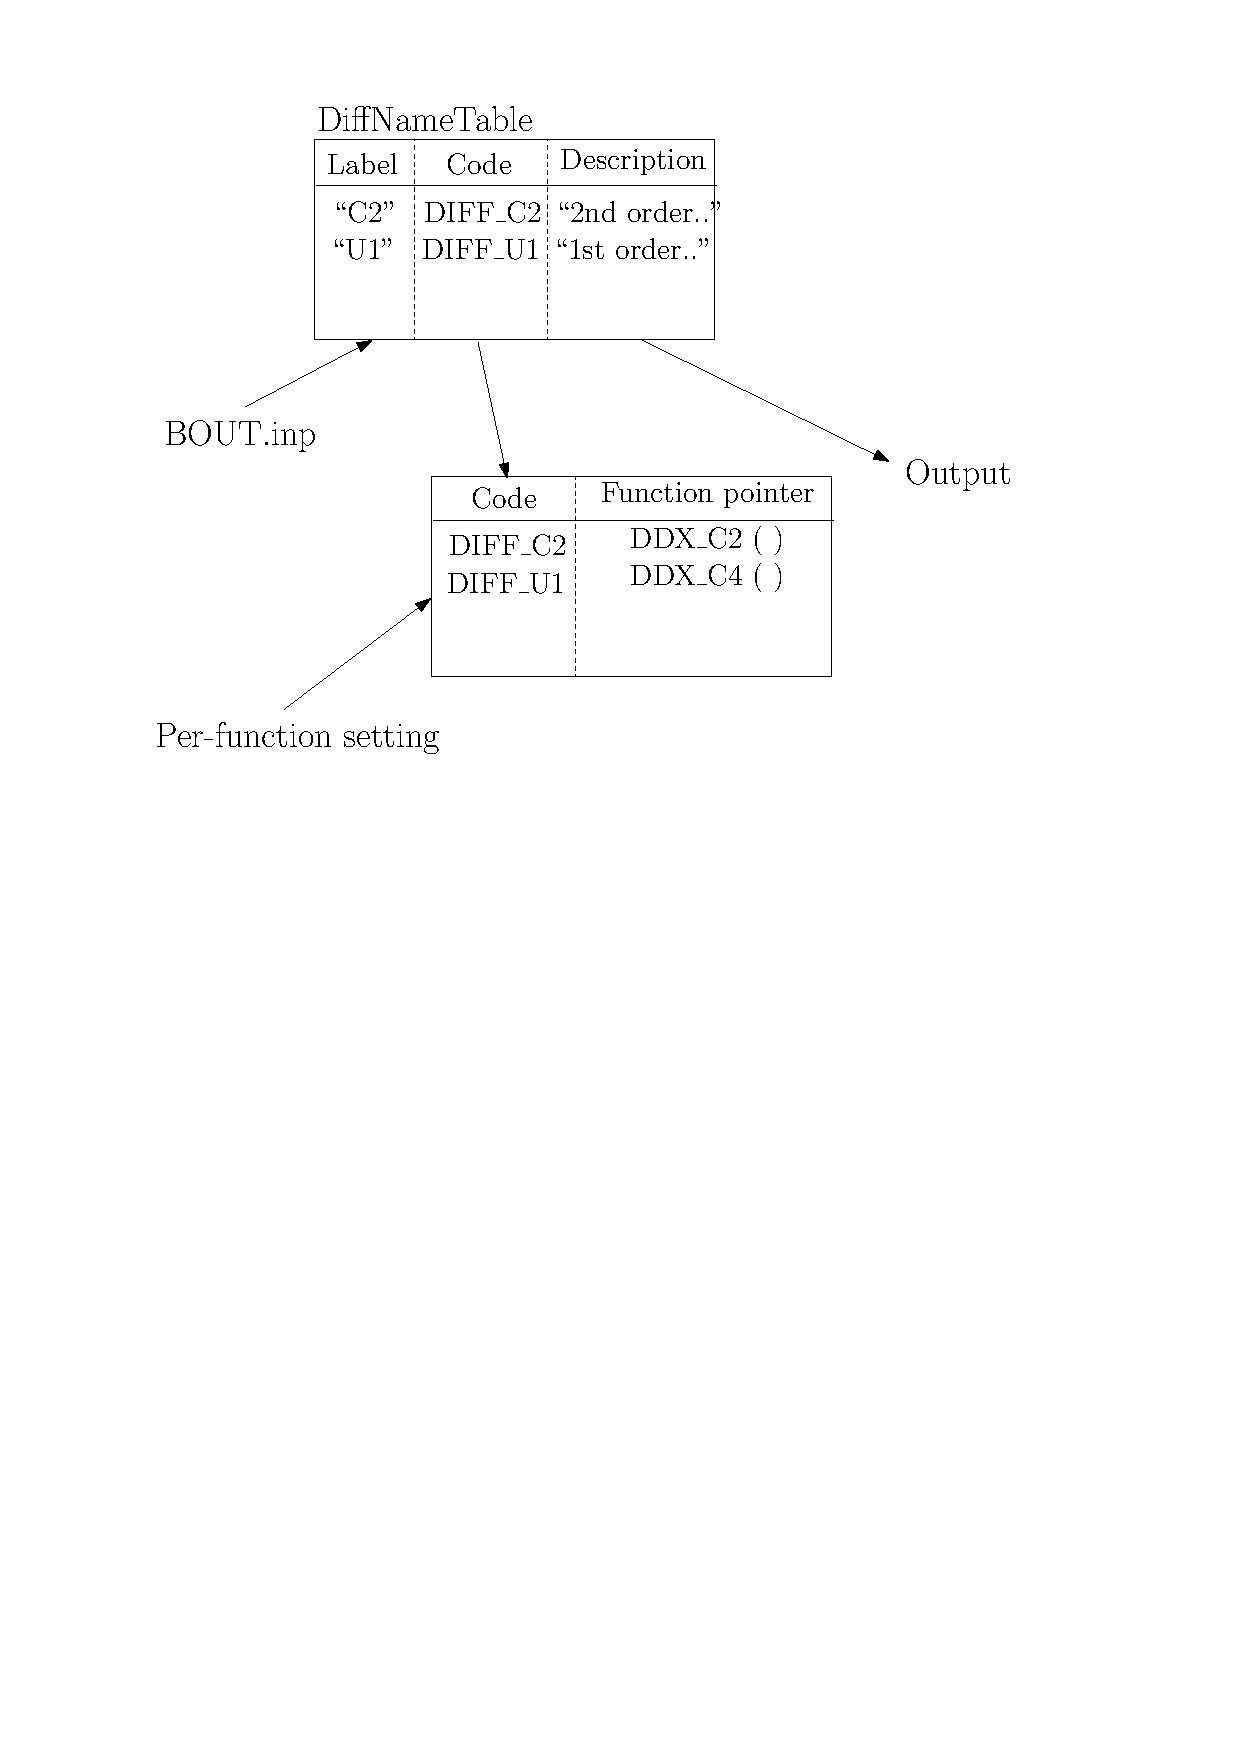
\includegraphics[scale=0.75]{figs/diffLookup.pdf}
\caption{Lookup tables for mapping between differential method labels, codes, descriptions and function pointers}
\label{fig:diffLookup}
\end{figure}

\subsection{Staggered grids}

\note{This feature is currently very experimental, and doesn't appear to work as it should}

By default, all quantities in BOUT++ are defined at cell centre, and
all derivative methods map cell-centred quantities to cell centres.
Switching on staggered grid support in BOUT.inp:
\begin{verbatim}
StaggerGrids = true
\end{verbatim}
allows quantities to be defined on cell boundaries. Functions such as \code{DDX} now have to handle
all possible combinations of input and output locations, in addition to the possible
derivative methods. 

Several things are not currently implemented, which probably should be:
\begin{itemize}
\item Only 3D fields currently have a cell location attribute. The location (cell centre etc) of 2D fields is ignored at the moment. The rationale for this is that 2D fields are assumed to be slowly-varying equilibrium quantities for which it won't matter so much. Still, needs to be improved in future
\item Twist-shift and X shifting still treat all quantities as cell-centred.
\item No boundary condition functions yet account for cell location. 
\end{itemize}

Currently, BOUT++ does not support values at cell corners; values can
only be defined at cell centre, or at the lower X,Y, or Z boundaries. 
This is 

Once staggered grids are enabled, two types of stencil are needed: those
which map between the same cell location (e.g. cell-centred values to cell-centred values), and those which map to different locations (e.g. cell-centred to lower X).

\begin{figure}[htb!]
\centering
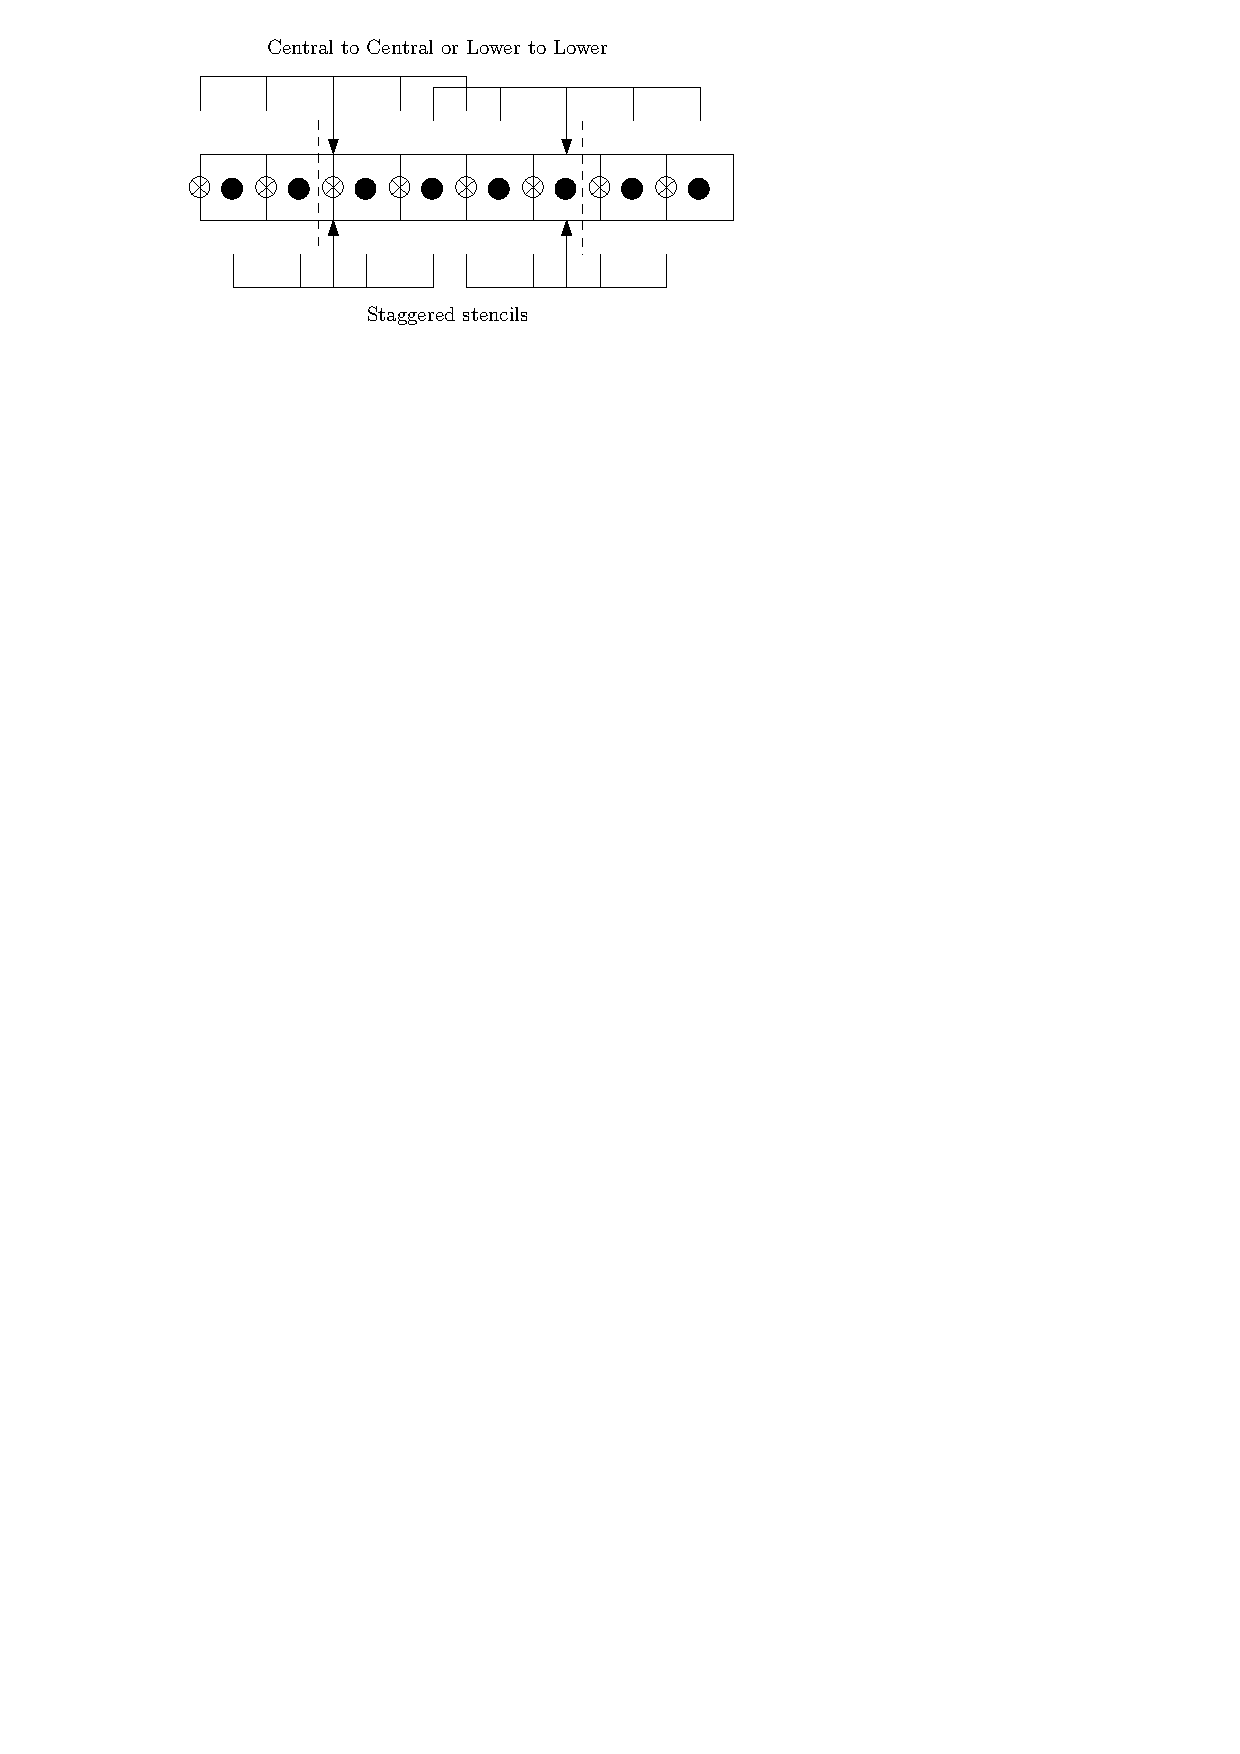
\includegraphics[scale=0.9]{figs/diffStencils.pdf}
\caption{Stencils with cell-centred (solid) and lower shifted values (open). Processor boundaries
marked by vertical dashed line}
\label{fig:diffStencils}
\end{figure}

Central differencing using 4-point stencil:
\begin{eqnarray*}
y &=& \left(9y_{-1/2} + 9y_{1/2} - y_{-3/2} - y_{3/2}\right) / 16 \\
\deriv{y}{x} &=& \left( 27y_{1/2} - 27y_{-1/2} - y_{3/2} + y_{-3/2}\right) / 24\Delta x \\
\frac{\partial^2 y}{\partial x^2} &=& \left(y_{3/2} + y_{-3/2} - y_{1/2} - y_{-1/2}\right) / 2\Delta x^2
\end{eqnarray*}

\note{What should the default cell location of a derivative be? Currently the default is to remain the same as without staggered grids. Setting \code{StaggerGrids = true} by itself has no effect - derivative output locations have to be explicitly set.}

\begin{table}[htbp!]
\caption{DDX actions depending on input and output locations. Uses first match.}
\label{tab:ddxloc}
\centering
\begin{tabular}[c]{c c | l}
\hline
Input & Output & Actions \\
\hline
\multicolumn{2}{c}{Same locations} & Central stencil \\
CENTRE & XLOW & Lower staggered stencil \\
XLOW & CENTRE & Upper staggered stencil \\
XLOW & Any & Staggered stencil to CENTRE, then interpolate \\
CENTRE & Any & Central stencil, then interpolate \\
Any & Any & Interpolate to centre, use central stencil, then interpolate \\
\hline
\end{tabular}
\end{table}

\section{Laplacian inversion}

\note{This part of the code needs some algorithm improvement (better parallel tridiagonal solver).}

Several different algorithms are implemented for Laplacian inversion, and
they differ between serial and parallel versions.
Serial inversion can currently either be done using a tridiagonal solver
(Thomas algorithm), or a band-solver (allowing $4^{th}$-order differencing).

\subsection{Thomas algorithm (serial)}

\subsection{Band solver (serial)}

This is band-solver which performs a $4^{th}$-order inversion. Currently this
is only available when \code{NXPE=1}; when more than one processor is used in $x$,
the Laplacian algorithm currently reverts to $3^{rd}$-order.

\subsection{Thomas algorithm (parallel)}

The current parallel code is a simple parallelisation of the Thomas algorithm
(so only 2nd order). The operations performed are the same as for the
serial code (useful for testing), but this means it is very inefficient.
Figure~\ref{fig:par_laplace} shows the useage of 4 processors inverting a set of 3 poloidal slices
(i.e. MYSUB=3)
\begin{figure}[htbp!]
\centering
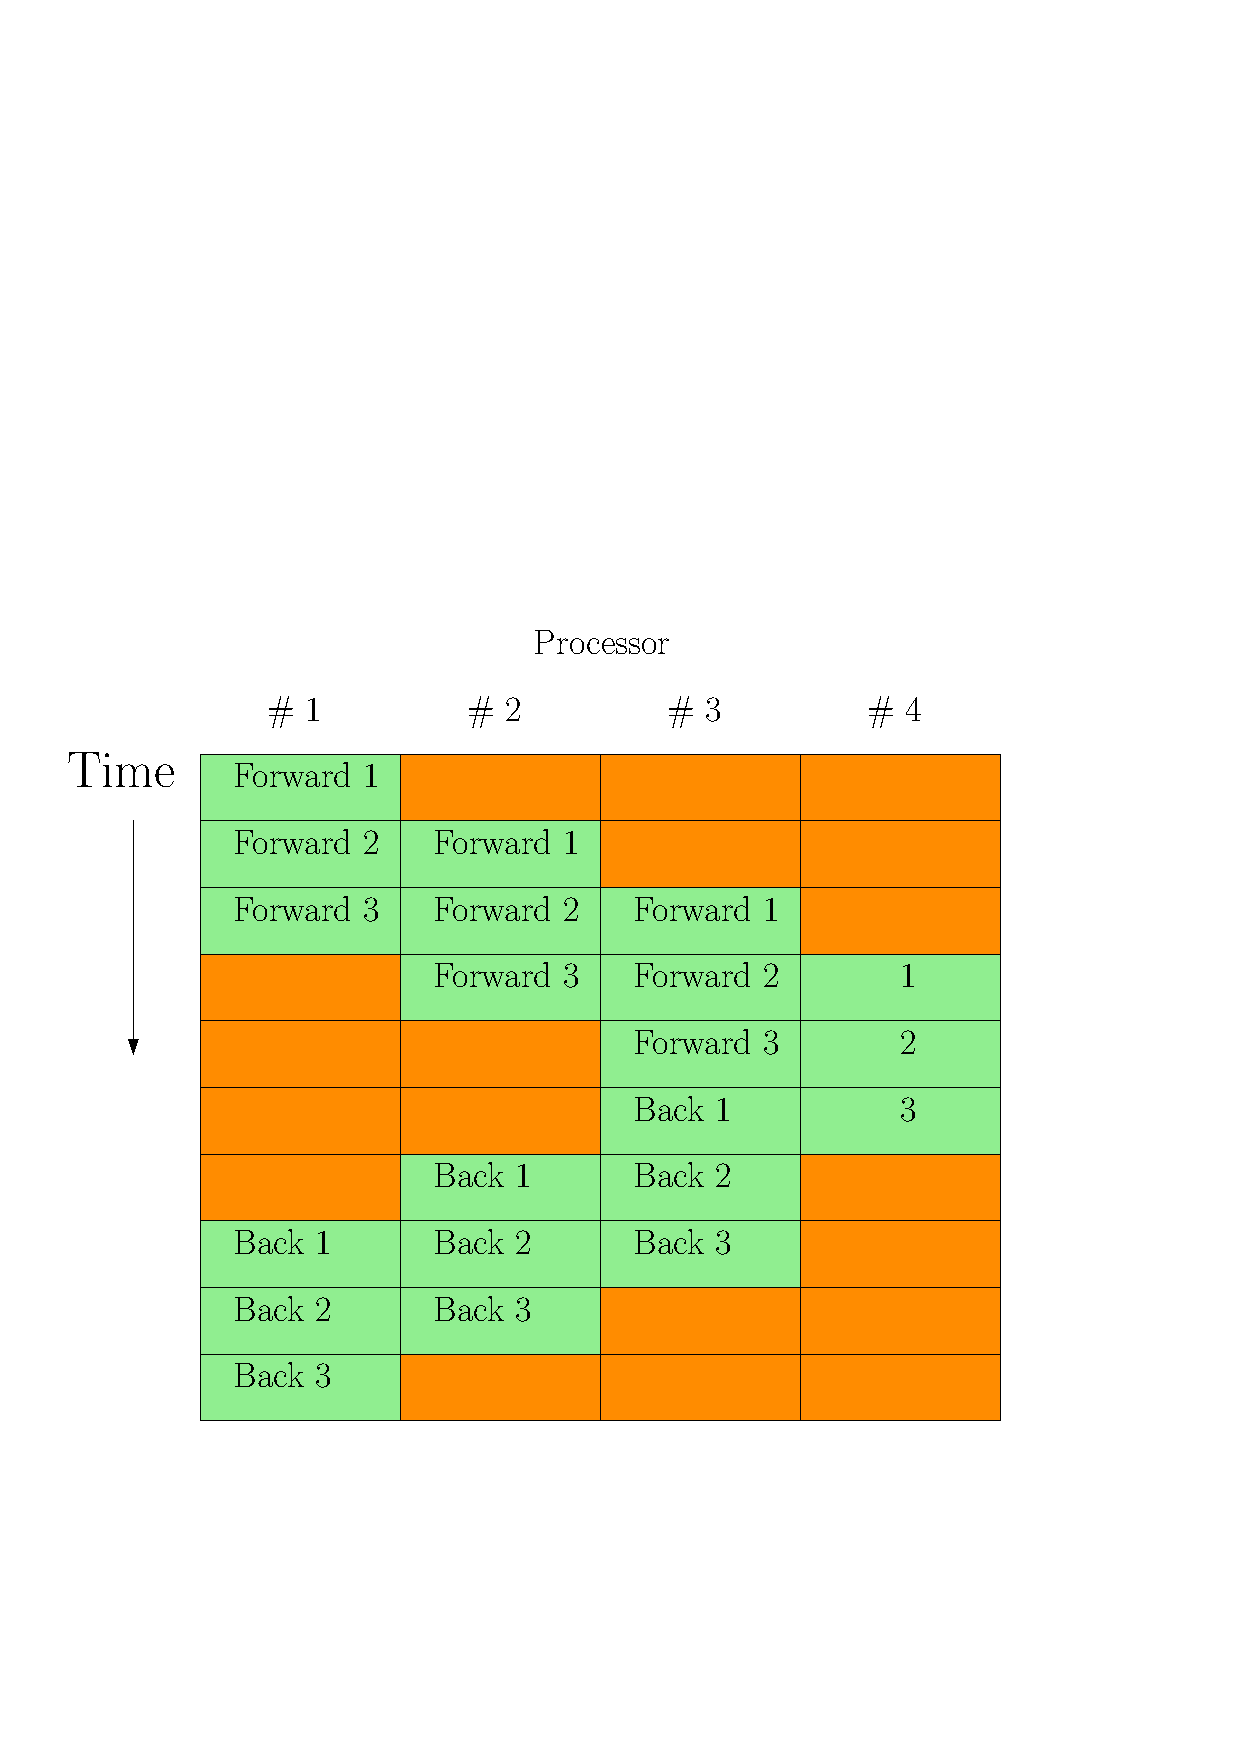
\includegraphics[width=0.5\paperwidth, keepaspectratio]{figs/par_laplace.pdf}
\caption{Parallel Laplacian inversion with MYSUB=3 on 4 processors. Red periods are where a processor is idle - in this case about 40\% of the time}
\label{fig:par_laplace}
\end{figure}

\subsection{PDD algorithm (parallel)}

This is the Parallel Diagonally Dominant (PDD) algorithm. It's very fast, but
achieves this by neglecting some cross-processor terms. For ELM simulations, it has
been found that these terms are important, so this method is not usually used. 

\section{Mesh}

The mesh is used in pretty much all parts of the code, and deals with 
things like the geometry of the mesh (metric tensors etc.), and how the
mesh is divided between processors (communications). The Mesh class
(\file{mesh/mesh.h}) defines an interface, whilst currently BoutMesh
(\file{mesh/boutmesh.h}) is the only implementation of this interface.

\subsection{Loading a mesh}

To load in a mesh from a file or other source, there are the commands:
\begin{lstlisting}
int addSource(GridDataSource);   // Add a data source
int load();                      // Load from added data sources
int load(GridDataSource);        // Load from specified data source
\end{lstlisting}
all of which return an error code (0 if successful). 
\code{addSource} is used to add a set of input data sources which
inherit from \code{GridDataSource}. \code{load()} loads the mesh
from these sources, querying each data source in turn for the required
variables (in the order in which they were added). \code{load(GridDataSource)}
loads the mesh from only the supplied data source.

In \file{bout++.cpp}, this is used to initialise the mesh:
\begin{lstlisting}
mesh->addSource(new GridFile(data_format(grid_name), grid_name));
if(mesh->load()) {
  output << "Failed to read grid. Aborting\n";
  return 1;
}
\end{lstlisting}
which creates a \code{GridFile} object based on the data format of 
the grid file name, then adds that as a source of data for Mesh.

For post-processing of the results, it's useful to have 
mesh quantities in the dump files along with the results. To do this,
there's the function
\begin{lstlisting}
void outputVars(Datafile &file); // Add mesh vars to file
\end{lstlisting}
which is called during BOUT++ initialisation.

\subsubsection{Implementation: BoutMesh}

BoutMesh class uses the BOUT indices (which trace back to UEDGE... there's
heritage here):
\begin{lstlisting}
int ixseps1, ixseps2, jyseps1_1, jyseps2_1, jyseps1_2, jyseps2_2;
\end{lstlisting}
\code{ixseps1} and \code{ixseps2} give the X location of the separatrices,
and are equal in the case of single-null configurations. The indexing
is such that all points \code{0 <= x < ixseps1} are inside the separatrix,
whilst \code{ixseps1 <= x < ngx} are outside.

\subsection{Index ranges}

The Mesh class includes several public members which describe the
size of the mesh, and are used all over BOUT++ to loop over variables:
\begin{lstlisting}
/// Size of the mesh on this processor including guard/boundary cells
int ngx, ngy, ngz;  
/// Local ranges of data (inclusive), excluding guard cells
int xstart, xend, ystart, yend;
\end{lstlisting}

\subsection{Getting data}

The \code{load()} code above needs to read data for the mesh, and physics
codes usually need to read their initial profiles during initialisation.
To do this, Mesh provides an overloaded function \code{get}:
\begin{lstlisting}
int get(var, const char *name); // Request data from mesh file
\end{lstlisting}
where \code{var} can be just about any BOUT++ datatype (\code{Field2D},
\code{Vector3D} etc.). 

\subsubsection{Implementation: BoutMesh}

For integers and reals, the implementation is fairly trivial. Uses
the Mesh protected functions to find a data source and read data from it.
\begin{lstlisting}
GridDataSource* s = findSource(name);  // Find a source of data
s->open(name);                          // Open the source
bool success = s->fetch(&ival, name);   // Get the data
s->close();                             // Close the source
\end{lstlisting}

To read 2D and 3D fields, the branch-cuts need to be taken into account.

\subsection{Communications}

The most common type of communication is to just exchange all
guard cells with neighboring processors. Mesh provides the following
commands for doing this:
\begin{lstlisting}
int communicate(FieldData, ...); // Communicate one or more fields
int communicate(FieldGroup);     // Communicate a group of fields
int communicate(FieldData);      // Returns error code
comm_handle send(FieldGroup);    // Send data
int wait(comm_handle);           // Receive data
\end{lstlisting}
\code{communicate(FieldData)} can (currently) be used to communicate
up to 4 variables together, and makes the code quite clear. For example in
\file{examples/DriftInstability/2fluid.cpp} around line 360:
\begin{lstlisting}
// Need to communicate jpar
mesh->communicate(jpar);
\end{lstlisting}
Since this uses the \code{FieldData} interface like Datafile, this can
be used to communicate all BOUT++ field data types. The limit of 4 is
because the C-style \code{varargs} system doesn't work with ``non POD''
variables, i.e. classes. To communicate a larger number of variables,
create a \code{FieldGroup} object to group fields together, then communicate
them all together:
\begin{lstlisting}
FieldGroup comgrp;  // Group of variables for communication
Field3D P;
Vector3D V;

comgrp.add(P); // Add the variables
comgrp.add(V); // Usually done in physics_init

mesh->communicate(comgrp); // Communicate in physics_run
\end{lstlisting}

If you want to overlap communications with calculations then
use the \code{send} and \code{wait} functions instead of \code{communicate}.
\begin{lstlisting}
comm_handle ch = mesh->send(comgrp); // Start the communications
// Calculations which don't need variables in comgrp
wait(ch); // Wait for all communications to finish
\end{lstlisting}

\subsubsection{Implementation: BoutMesh}

In BoutMesh, the communication is controlled by the variables
\begin{lstlisting}
int UDATA_INDEST, UDATA_OUTDEST, UDATA_XSPLIT;
int DDATA_INDEST, DDATA_OUTDEST, DDATA_XSPLIT;
int IDATA_DEST, ODATA_DEST;
\end{lstlisting}
In the Y direction, each boundary region ({\bf U}p and {\bf D}own in Y) 
can be split into two, with \code{0 <= x < UDATA\_XSPLIT} going to
the processor index \code{UDATA\_INDEST}, and \code{UDATA\_INDEST <= x < ngx}
going to \code{UDATA\_OUTDEST}. Similarly for the Down boundary.
Since there are no branch-cuts in the X direction, there is just one
destination for the {\bf I}nner and {\bf O}uter boundaries.
In all cases a negative processor number means that there's a domain boundary.

\subsection{X communications}

For parallel Laplacian inversions, communication is needed in the X
direction only, and involves quantities which are not in Fields.

\begin{lstlisting}
bool firstX();  // True if at the inner X boundary
bool lastX();   // True if at the outer X boundary
int NXPE, PE_XIND; // Number of processors in X, and X processor index
int sendXOut(real *buffer, int size, int tag);
sendXIn(real *buffer, int size, int tag);
comm_handle irecvXOut(real *buffer, int size, int tag);
comm_handle irecvXIn(real *buffer, int size, int tag);
\end{lstlisting}

The variables \code{NXPE} and \code{PE\_XIND} shouldn't really be there,
but are currently needed because the SPT algorithm in \file{invert\_laplace.cpp}
needs to know when it's going to be next and so keep track of which processor
number is currently working. This logic to pass a problem along a chain in
X should really be moved into Mesh.

\subsection{Y-Z surface communications}

\begin{lstlisting}
SurfaceIter* iterateSurfaces();
const Field2D averageY(const Field2D &f); // Average in Y
bool surfaceClosed(int jx, real &ts); // Test if a surface is closed, and if so get the twist-shift angle
\end{lstlisting}

\subsection{Boundary regions}

The boundary condition code (see section~\ref{sec:boundaries}) needs
ways to loop over the boundary regions, without needing to know
the details of the mesh.

\begin{lstlisting}
// Boundary region iteration
RangeIter* iterateBndryLowerY();
RangeIter* iterateBndryUpperY();

bool BoundaryOnCell; // NB: DOESN'T REALLY BELONG HERE
\end{lstlisting}
  
The \code{RangeIter} class is a simple iterator
\begin{lstlisting}
class RangeIter {
 public:
  virtual void first() = 0;
  virtual void next() = 0;
  virtual bool isDone() = 0;
  
  int ind; // The index
};
\end{lstlisting}
which allows looping over the X indices in the boundary. For example, in
\code{boundary.cpp} to loop over the upper Y boundary of a 2D variable
\code{var}:
\begin{lstlisting}
RangeIter* xr = mesh->iterateBndryUpperY(); // Upper boundary
for(xr->first(); !xr->isDone(); xr->next())
  for(int jy=mesh->yend+1;jy<mesh->ngy;jy++) {
    var[xr->ind][jy] = ...
  }
\end{lstlisting}

\subsection{Initial profiles}

The initial profiles code needs to construct a solution which is smooth
everywhere, with a form of perturbation specified in the input file
for each direction. In order to do this, it needs a continuous function
to use as an index. This is supplied by the functions:
\begin{lstlisting}
real GlobalX(int jx); // Continuous X index between 0 and 1
real GlobalY(int jy); // Continuous Y index (0 -> 1)
\end{lstlisting}
which take a local x or y index and return a globally continuous x or y
index.

\subsection{Differencing}

The mesh spacing is given by the public members
\begin{lstlisting}
// These used for differential operators 
Field2D dx, dy;
Field2D d2x, d2y;    // 2nd-order correction for non-uniform meshes		
real zlength, dz;    // Derived from options (in radians)
\end{lstlisting}

\subsection{Metrics}

The contravariant and covariant metric tensor components are
public members of \code{Mesh}:
\begin{lstlisting}
// Contravariant metric tensor (g^{ij})
Field2D g11, g22, g33, g12, g13, g23; // These are read in grid.cpp

// Covariant metric tensor
Field2D g_11, g_22, g_33, g_12, g_13, g_23;

int calcCovariant();     // Invert contravatiant metric to get covariant
int calcContravariant(); // Invert covariant metric to get contravariant
\end{lstlisting}
If only one of these sets is modified by an external code, then
\code{calc\_covariant} and \code{calc\_contravariant} can be used
to calculate the other (uses Gauss-Jordan currently).

From the metric tensor components, Mesh calculates several other useful
quantities:
\begin{lstlisting}
int jacobian(); // Calculate J and Bxy
Field2D J; // Jacobian
Field2D Bxy; // Magnitude of B = nabla z times nabla x

/// Calculate differential geometry quantities from the metric tensor
int geometry();

// Christoffel symbol of the second kind (connection coefficients)
Field2D G1_11, G1_22, G1_33, G1_12, G1_13;
Field2D G2_11, G2_22, G2_33, G2_12, G2_23;
Field2D G3_11, G3_22, G3_33, G3_13, G3_23;
  
Field2D G1, G2, G3;
\end{lstlisting}

These quantities are public and accessible everywhere, but this is because
they are needed in a lot of the code. They shouldn't change
after initialisation, unless the physics model starts doing fancy things with
deforming meshes.

\subsection{Miscellaneous}

There are some public members of Mesh which are there for some specific
task and don't really go anywhere else (yet). 

To perform radial derivatives in tokamak geometry, interpolation is needed
in the Z direction. This is done by shifting in Z by a phase factor, performing
the derivatives, then shifting back. The following public variables are currently
used for this:
\begin{lstlisting}
bool ShiftXderivs; // Use shifted X derivatives
int  ShiftOrder;   // Order of shifted X derivative interpolation
Field2D zShift;    // Z shift for each point (radians)
  
Field2D ShiftTorsion; // d <pitch angle> / dx. Needed for vector differentials (Curl)
Field2D IntShiftTorsion; // Integrated shear (I in BOUT notation)
bool IncIntShear; // Include integrated shear (if shifting X)
\end{lstlisting}

\begin{lstlisting}
int  TwistOrder;   // Order of twist-shift interpolation
\end{lstlisting}
This determines what order method to use for the interpolation at the twist-shift
location, with \code{0} meaning FFT during communication. Since this must be 0 at the moment
it's fairly redundant and should be removed.

A (currently experimental) feature is 
\begin{lstlisting}
bool StaggerGrids;    ///< Enable staggered grids (Centre, Lower). Otherwise all vars are cell centred (default).
\end{lstlisting}

\section{Boundary conditions}
\label{sec:boundaries}

The boundary condition system needs to be very flexible in order to handle:
\begin{itemize}
\item Meshes which can divide up the boundary into an arbitrary number
  of regions, giving each one a label. For example in BoutMesh 
  (specific to tokamaks), the boundary regions are labelled "core",
  "sol", "pf" and "target".
\item Each variable can have a different boundary condition in each region.
  It should be possible to have a global setting "all variables have dirichlet
  conditions on all boundaries", which is over-ridden by more specific settings
  such as "All variables have neumann conditions on the inner x boundaries", 
  and finally to "variable 'Ni' has laplacian boundary conditions in the
  'sol' regions"
\item Boundary conditions can be modified to be ``relaxing''. This means that
  rather than enforcing a strict boundary condition, it's a mixture of
  zero-gradient in the time-derivative combined with a damping (relaxation)
  towards the desired boundary condition. This can help improve the numerics
  of turbulence simulations.
\item Users should be able to implement their own boundary conditions,
  and add them to the system at run-time without modifying the core code.
\item After \code{physics\_init}, a boundary condition must be applied to
  the variables. During a simulation (at the end of \code{physics\_run}),
  boundary conditions need to be applied to the time-derivatives. The
  boundary system should ensure that these conditions are consistent.
\end{itemize}

\subsection{Boundary regions}
\label{sec:BoundaryRegion}

Different regions of the boundary such as ``core'', ``sol'' etc. are
labelled by the \code{Mesh} class (i.e. \code{BoutMesh}), which
implements a member function defined in \file{mesh.h}:
\begin{lstlisting}[firstnumber=150]
  // Boundary regions
  virtual vector<BoundaryRegion*> getBoundaries() = 0;
\end{lstlisting}
This returns a vector of pointers to \code{BoundaryRegion} objects,
each of which describes a boundary region with a label, a \code{BndryLoc} 
location (i.e. inner x, outer x, lower y, upper y or all), and iterator
functions for looping over the points. This class is
defined in \file{boundary\_region.h}:
\begin{lstlisting}[firstnumber=12]
/// Describes a region of the boundary, and a means of iterating over it
class BoundaryRegion {
  public:
  BoundaryRegion();
  BoundaryRegion(const string &name, int xd, int yd);
  virtual ~BoundaryRegion();
  
  string label; // Label for this boundary region
  
  BndryLoc location; // Which side of the domain is it on?
  
  int x,y; // Indices of the point in the boundary
  int bx, by; // Direction of the boundary [x+dx][y+dy] is going outwards

  virtual void first() = 0;
  virtual void next() = 0; // Loop over every element from inside out (in X or Y first)
  virtual void nextX() = 0; // Just loop over X
  virtual void nextY() = 0; // Just loop over Y
  virtual bool isDone() = 0; // Returns true if outside domain. Can use this with nested nextX, nextY
};
\end{lstlisting}

{\bf Example:} To loop over all points in \code{BoundaryRegion *bndry} , use
\begin{lstlisting}[numbers=none]
  for(bndry->first(); !bndry->isDone(); bndry->next()) {
    ...
  }
\end{lstlisting}
Inside the loop, \code{bndry->x} and \code{bndry->y} are the indices
of the point, whilst \code{bndry->bx} and \code{bndry->by} are unit vectors
out of the domain. The loop is over all the points from the domain outwards 
i.e. the point
\code{[bndry->x - bndry->bx][bndry->y - bndry->by]} will always be defined.

Sometimes it's useful to be able to loop over just one direction along the
boundary. To do this, it is possible to use \code{nextX()} or \code{nextY()}
rather than \code{next()}. It is also possible to loop over both dimensions
using:
\begin{lstlisting}[numbers=none]
  for(bndry->first(); !bndry->isDone(); bndry->nextX())
    for(; !bndry->isDone(); bndry->nextY()) {
      ...
    }
\end{lstlisting}

\subsection{Boundary operations}

On each boundary, conditions must be specified for each variable. 
The different conditions are imposed by \code{BoundaryOp} objects.
These set the values in the boundary region such that they obey e.g.
Dirichlet or Neumann conditions. The \code{BoundaryOp} class is defined
in \file{boundary\_op.h}:
\begin{lstlisting}[firstnumber=21]
/// An operation on a boundary
class BoundaryOp {
 public:
  BoundaryOp() {bndry = NULL;}
  BoundaryOp(BoundaryRegion *region)
  
  // Note: All methods must implement clone, except for modifiers (see below)
  virtual BoundaryOp* clone(BoundaryRegion *region, const list<string> &args);
  
  /// Apply a boundary condition on field f
  virtual void apply(Field2D &f) = 0;
  virtual void apply(Field3D &f) = 0;
  
  virtual void apply(Vector2D &f);
  
  virtual void apply(Vector3D &f);

  /// Apply a boundary condition on ddt(f)
  virtual void apply_ddt(Field2D &f);
  virtual void apply_ddt(Field3D &f);
  virtual void apply_ddt(Vector2D &f);
  virtual void apply_ddt(Vector3D &f);
  
  BoundaryRegion *bndry;
};
\end{lstlisting}
(where the implementations have been removed for clarity). 
Which has a pointer to a \code{BoundaryRegion} object specifying which
region this boundary is operating on.

Boundary conditions need to be imposed on the initial conditions (after
\code{physics\_init()}), and on the time-derivatives
(after \code{physics\_run()}). The \code{apply()} functions are therefore
called during initialisation and given the evolving variables, whilst the
\code{apply\_ddt} functions are passed the time-derivatives.

To implement a boundary operation, as a minimum the \code{apply(Field2D)}, 
\code{apply(Field2D)} and \code{clone()} need to be implemented: By default
the \code{apply(Vector)} will call the \code{apply(Field)} functions on each
component individually, and the \code{apply\_ddt()} functions just call
the \code{apply()} functions.

{\bf Example}: Neumann boundary conditions are defined in
\file{boundary\_standard.h}:
\begin{lstlisting}[firstnumber=22]
/// Neumann (zero-gradient) boundary condition
class BoundaryNeumann : public BoundaryOp {
 public:
  BoundaryNeumann() {}
 BoundaryNeumann(BoundaryRegion *region):BoundaryOp(region) { }
  BoundaryOp* clone(BoundaryRegion *region, const list<string> &args);
  void apply(Field2D &f);
  void apply(Field3D &f);
};
\end{lstlisting}
and implemented in \file{boundary\_standard.cpp}
\begin{lstlisting}[firstnumber=52]
void BoundaryNeumann::apply(Field2D &f)
{
  // Loop over all elements and set equal to the next point in
  for(bndry->first(); !bndry->isDone(); bndry->next())
    f[bndry->x][bndry->y] = f[bndry->x - bndry->bx][bndry->y - bndry->by];
}

void BoundaryNeumann::apply(Field3D &f)
{
  for(bndry->first(); !bndry->isDone(); bndry->next())
    for(int z=0;z<mesh->ngz;z++)
      f[bndry->x][bndry->y][z] = f[bndry->x - bndry->bx][bndry->y - bndry->by][z];
}
\end{lstlisting}
This is all that's needed in this case since there's no difference between
applying Neumann conditions to a variable and to its time-derivative, 
and Neumann conditions for vectors are just Neumann conditions
on each vector component. 

To create a boundary condition, we need to give it a boundary region
to operate over:
\begin{lstlisting}[numbers=none]
BoundaryRegion *bndry = ...
BoundaryOp op = new BoundaryOp(bndry);
\end{lstlisting}

The \code{clone} function is used to create
boundary operations given a single object as a template
in \code{BoundaryFactory}. This can take additional arguments
as a vector of strings - see explanation in section~\ref{sec:BoundaryFactory}.

\subsection{Boundary modifiers}

To create more complicated boundary conditions from simple ones (such as
Neumann conditions above), boundary operations can be modified by
wrapping them up in a \code{BoundaryModifier} object, defined
in \file{boundary\_op.h}:
\begin{lstlisting}[firstnumber=63]
class BoundaryModifier : public BoundaryOp {
 public:
  virtual BoundaryOp* clone(BoundaryOp *op, const list<string> &args) = 0;
 protected:
  BoundaryOp *op;
};
\end{lstlisting}
Since \code{BoundaryModifier} inherits from \code{BoundaryOp}, 
modified boundary operations are just a different boundary operation and can
be treated the same (Decorator pattern). Boundary modifiers could also be
nested inside each other to create even more complicated boundary operations.
Note that the \code{clone} function is different to the \code{BoundaryOp} one:
instead of a \code{BoundaryRegion} to operate on, modifiers are passed a
\code{BoundaryOp} to modify.

Currently the only modifier is \code{BoundaryRelax}, defined in
\file{boundary\_standard.h}:
\begin{lstlisting}[firstnumber=64]
/// Convert a boundary condition to a relaxing one
class BoundaryRelax : public BoundaryModifier {
 public:
  BoundaryRelax(BoutReal rate) {r = fabs(rate);}
  BoundaryOp* clone(BoundaryOp *op, const list<string> &args);
  
  void apply(Field2D &f);
  void apply(Field3D &f);
  
  void apply_ddt(Field2D &f);
  void apply_ddt(Field3D &f);
 private:
  BoundaryRelax() {} // Must be initialised with a rate
  BoutReal r;
};
\end{lstlisting}

\subsection{Boundary factory}
\label{sec:BoundaryFactory}

The boundary factory creates new boundary operations from input strings,
for example turning "relax(dirichlet)" into a relaxing Dirichlet boundary
operation on a given region. It is defined in \file{boundary\_factory.h}
as a Singleton, so to get a pointer to the boundary factory use
\begin{lstlisting}[numbers=none]
  BoundaryFactory *bfact = BoundaryFactory::getInstance();
\end{lstlisting}
and to delete this singleton, free memory and cleanup at the end use:
\begin{lstlisting}[numbers=none]
  BoundaryFactory::cleanup();
\end{lstlisting}

Because users should be able to add new boundary conditions during
\code{physics\_init()}, boundary conditions are not hard-wired into
\code{BoundaryFactory}. Instead, boundary conditions must be registered
with the factory, passing an instance which can later be cloned. This
is done in \file{bout++.cpp} for the standard boundary conditions:
\begin{lstlisting}[firstnumber=258]
  BoundaryFactory* bndry = BoundaryFactory::getInstance();
  bndry->add(new BoundaryDirichlet(), "dirichlet");
  ...
  bndry->addMod(new BoundaryRelax(10.), "relax");
\end{lstlisting}
where the \code{add} function adds BoundaryOp objects, whereas
\code{addMod} adds \code{BoundaryModifier} objects. {\bf Note}: The
objects passed to \code{BoundaryFactory} will be deleted when \code{cleanup()}
is called. 

When a boundary operation is added, it is given a name
such as ``dirichlet'', and similarly for the modifiers (``relax'' above).
These labels and object pointers are stored internally in \code{BoundaryFactory}
in maps defined in \file{boundary\_factory.h}:
\begin{lstlisting}[firstnumber=43]
  // Database of available boundary conditions and modifiers
  map<string, BoundaryOp*> opmap;
  map<string, BoundaryModifier*> modmap;
\end{lstlisting}
These are then used by \code{BoundaryFactory::create()}:
\begin{lstlisting}[firstnumber=24]
  /// Create a boundary operation object
  BoundaryOp* create(const string &name, BoundaryRegion *region);
  BoundaryOp* create(const char* name, BoundaryRegion *region);
\end{lstlisting}
to turn a string such as ``relax(dirichlet)'' and a \code{BoundaryRegion}
pointer into a \code{BoundaryOp} object. These functions are implemented
in \file{boundary\_factory.cpp}, starting around line 42. The parsing is
done recursively by matching the input string to one of:
\begin{itemize}
\item \code{modifier(<expression>, arg1, ...)}
\item \code{modifier(<expression>)}
\item \code{operation(arg1, ...)}
\item \code{operation}
\end{itemize}
the \code{<expression>} variable is then resolved into a BoundaryOp
object by calling \code{create(<expression, region)}.

When an operator or modifier is found, it is created from the pointer
stored in the \code{opmap} or \code{modmap} maps using the
\code{clone} method, passing
a \code{list<string>} reference containing any arguments. It's up
to the operation implementation to ensure that the correct number of
arguments are passed, and to parse them into floats or other types.

{\bf Example}: The Dirichlet boundary condition can take an optional
argument to change the value the boundary's set to. In \file{boundary\_standard.cpp}:
\begin{lstlisting}[firstnumber=13]
BoundaryOp* BoundaryDirichlet::clone(BoundaryRegion *region, const list<string> &args)
{
  if(!args.empty()) {
    // First argument should be a value
    stringstream ss;
    ss << args.front();
    
    BoutReal val;
    ss >> val;
    return new BoundaryDirichlet(region, val);
  }
  return new BoundaryDirichlet(region);
}
\end{lstlisting}
If no arguments are passed i.e. the string was ``dirichlet'' or ``dirichlet()''
then the \code{args} list is empty, and the default value (0.0) is used.
If one or more arguments is used then the first argument is parsed into a
\code{BoutReal} type and used to create a new \code{BoundaryDirichlet} object.
If more arguments are passed then these are just ignored; probably a warning
should be printed.

To set boundary conditions on a field, \code{FieldData} methods are
defined in \file{field\_data.h}:
\begin{lstlisting}
// Boundary conditions
  void setBoundary(const string &name); ///< Set the boundary conditions
  void setBoundary(const string &region, BoundaryOp *op); ///< Manually set
  virtual void applyBoundary() {}
  virtual void applyTDerivBoundary() {};
 protected:
  vector<BoundaryOp*> bndry_op; // Boundary conditions
\end{lstlisting}
The \code{setBoundary(const string \&name)} method is implemented in
\file{field\_data.cpp}. It first gets a vector of pointers to
\code{BoundaryRegion}s from the mesh, then loops over these calling
\code{BoundaryFactory::createFromOptions} for each one and adding the resulting
boundary operator to the \code{bndry\_op} vector.


\section{Solver}

The solver is the interface between BOUT++ and the time-integration code
such as SUNDIALS. All solvers implement the \code{Solver} class
interface (see \file{src/solver/generic\_solver.h}).

First all the fields which are to be evolved need to be added
to the solver. These are always done in pairs, the first
specifying the field, and the second the time-derivative:
\begin{lstlisting}
void add(Field2D &v, Field2D &F_v, const char* name);
\end{lstlisting}
This is normally called in the \code{physics\_init} initialisation routine.
Some solvers (e.g. IDA) can support constraints, which need to be added
in the same way as evolving fields:
\begin{lstlisting}
bool constraints();
void constraint(Field2D &v, Field2D &C_v, const char* name);
\end{lstlisting}
The \code{constraints()} function tests whether or not the current
solver supports constraints. The format of \code{constraint(...)} is
the same as \code{add}, except that now the solver will attempt to make
\code{C\_v} zero. If \code{constraint} is called when the solver doesn't
support them then an error should occur.

If the physics model implements a preconditioner or Jacobian-vector
multiplication routine, these can be passed to the solver during
initialisation:
\begin{lstlisting}
typedef int (*PhysicsPrecon)(real t, real gamma, real delta);
void setPrecon(PhysicsPrecon f); // Specify a preconditioner
typedef int (*Jacobian)(real t);
void setJacobian(Jacobian j); // Specify a Jacobian
\end{lstlisting}
If the solver doesn't support these functions then the calls 
will just be ignored.

Once the problem to be solved has been specified, the solver can be
initialised using:
\begin{lstlisting}
int init(rhsfunc f, int argc, char **argv, bool restarting, int nout, real tstep);
\end{lstlisting}
which returns an error code (0 on success). This is currently
called in \file{bout++.cpp}:
\begin{lstlisting}
if(solver.init(physics_run, argc, argv, restart, NOUT, TIMESTEP)) {
  output.write("Failed to initialise solver. Aborting\n");
  return(1);
}
\end{lstlisting}
which passes the (physics module) RHS function \code{physics\_run}
to the solver along with the number and size of the output steps.

To run the solver using the (already supplied) settings, there is
the function:
\begin{lstlisting}
typedef int (*MonitorFunc)(real simtime, int iter, int NOUT);
int run(MonitorFunc f);
\end{lstlisting}

\subsection{Implementation: PVODE}


\subsection{Implementation: IDA}

\subsection{Implementation: PETSc}

\section{File I/O}

BOUT++ needs to deal with binary format files to read the grid;
read and write restart restart files; and write dump files. 
The two parts of the code which need to read and write data are therefore
the grid routines (\code{grid.h} and \code{grid.cpp}), and the
\code{Datafile} class (\code{datafile.h} and \code{datafile.cpp}).
All other parts which need to read or write data go through these
methods.

Several different file formats are commonly used, such as HDF, HDF5, and netCDF. 
For historical reasons (inherited from BOUT), BOUT++ originally used the
Portable Data Binary (PDB) format developed at LLNL. 
To separate the basic file format functions from the higher level grid and 
Datafile classes, these use an abstract class \code{DataFormat}. Any
class which implements the functions listed in \code{dataformat.h}
can therefore be passed to grid or datafile. This makes implementing
a new file format, and switching between formats at run-time, 
relatively straightforward.


Access to data in files is provided using a Bridge pattern: The
\code{Datafile} class provides an interface to the rest of the code
to read and write variables, whilst file formats implement the
\code{Dataformat} interface.
\begin{lstlisting}
class Datafile {
 public:
  Datafile();
  Datafile(DataFormat *format);
  ~Datafile();
  
  /// Set the file format by passing an interface class
  void setFormat(DataFormat *format);

  void setLowPrecision(); ///< Only output floats

  void add(var, const char *name, int grow = 0);

  int read(const char *filename, ...);
  int write(const char *filename, ...);
  int append(const char *filename, ...);
  bool write(const string &filename, bool append=false);

  /// Set this to false to switch off all data writing
  static bool enabled;
};
\end{lstlisting}


The important bits of the DataFormat interface are:
\begin{lstlisting}
class DataFormat {
 public:
  bool openr(const char *name);
  bool openw(const char *name, bool append=false);
  
  bool is_valid();
  
  void close();
  
  const char* filename();

  const vector<int> getSize(const char *var);
  const vector<int> getSize(const string &var);

  // Set the origin for all subsequent calls
  bool setOrigin(int x = 0, int y = 0, int z = 0); 
  bool setRecord(int t); // negative -> latest
  
  // Read / Write simple variables up to 3D

  bool read(int *var, const char *name, int lx = 1, int ly = 0, int lz = 0);
  bool read(real *var, const char *name, int lx = 1, int ly = 0, int lz = 0);

  bool write(int *var, const char *name, int lx = 0, int ly = 0, int lz = 0);
  bool write(real *var, const char *name, int lx = 0, int ly = 0, int lz = 0);

  // Read / Write record-based variables

  bool read_rec(int *var, const char *name, int lx = 1, int ly = 0, int lz = 0);
  bool read_rec(real *var, const char *name, int lx = 1, int ly = 0, int lz = 0);

  bool write_rec(int *var, const char *name, int lx = 0, int ly = 0, int lz = 0);
  bool write_rec(real *var, const char *name, int lx = 0, int ly = 0, int lz = 0);

  // Optional functions
  
  void setLowPrecision();
};
\end{lstlisting}

\section{Miscellaneous}

Other small modules which don't really fit into any system, but are needed.


\subsection{Printing messages}



\subsection{Reading input options}



\subsection{Error handling}


\end{document}

